
%% bare_jrnl_compsoc.tex
%% V1.4b
%% 2015/08/26
%% by Michael Shell
%% See:
%% http://www.michaelshell.org/
%% for current contact information.
%%
%% This is a skeleton file demonstrating the use of IEEEtran.cls
%% (requires IEEEtran.cls version 1.8b or later) with an IEEE
%% Computer Society journal paper.
%%
%% Support sites:
%% http://www.michaelshell.org/tex/ieeetran/
%% http://www.ctan.org/pkg/ieeetran
%% and
%% http://www.ieee.org/

%%*************************************************************************
%% Legal Notice:
%% This code is offered as-is without any warranty either expressed or
%% implied; without even the implied warranty of MERCHANTABILITY or
%% FITNESS FOR A PARTICULAR PURPOSE! 
%% User assumes all risk.
%% In no event shall the IEEE or any contributor to this code be liable for
%% any damages or losses, including, but not limited to, incidental,
%% consequential, or any other damages, resulting from the use or misuse
%% of any information contained here.
%%
%% All comments are the opinions of their respective authors and are not
%% necessarily endorsed by the IEEE.
%%
%% This work is distributed under the LaTeX Project Public License (LPPL)
%% ( http://www.latex-project.org/ ) version 1.3, and may be freely used,
%% distributed and modified. A copy of the LPPL, version 1.3, is included
%% in the base LaTeX documentation of all distributions of LaTeX released
%% 2003/12/01 or later.
%% Retain all contribution notices and credits.
%% ** Modified files should be clearly indicated as such, including  **
%% ** renaming them and changing author support contact information. **
%%*************************************************************************


% *** Authors should verify (and, if needed, correct) their LaTeX system  ***
% *** with the testflow diagnostic prior to trusting their LaTeX platform ***
% *** with production work. The IEEE's font choices and paper sizes can   ***
% *** trigger bugs that do not appear when using other class files.       ***                          ***
% The testflow support page is at:
% http://www.michaelshell.org/tex/testflow/


\documentclass[10pt,journal,compsoc]{IEEEtran}
%
% If IEEEtran.cls has not been installed into the LaTeX system files,
% manually specify the path to it like:
% \documentclass[10pt,journal,compsoc]{../sty/IEEEtran}



\usepackage{booktabs} % For formal tables
\usepackage{listings}
\usepackage{balance}
\usepackage{lipsum}
\usepackage{algorithm}
\usepackage{algorithmic}
\usepackage{dsfont}
\usepackage{titlecaps}
\usepackage{array}
\usepackage{tabularx}
\usepackage{fancyvrb}
\usepackage{amsmath}
\usepackage{amssymb}
\usepackage{stmaryrd}
\usepackage{tikz}
\usepackage{pgfplots}
\usepackage{pgfplotstable}
\usepgfplotslibrary{colorbrewer}
\usetikzlibrary{shadows}
\usetikzlibrary{arrows}
\usetikzlibrary{arrows.meta}
\usetikzlibrary{shadows.blur}


\tikzset{%
   tipSq/.tip={Square[open,fill=black]}
}

\pgfplotsset{cycle list/BrBG}


\newcommand{\red}[1] {\textcolor{red} {#1}} 

\DeclareMathOperator*{\concur}{\parallel}

\DeclareMathOperator*{\argmax}{arg\,max}

\definecolor{prismgreen}{rgb}{0, 0.6, 0}
\definecolor{haiqprocblue}{rgb}{0, 0.0, 0.6}

\lstdefinelanguage{haiq}{
  keywords={%
      assert, pred, all, no, lone, one, some, check, run,
      but, let, implies, not, iff, in, and, or, set, sig, Int, int,
      if, then, else, exactly, disj, fact, fun, module, abstract,
      extends, open, none, univ, iden, seq,
      init, var, enum, formula, false, true, bool, 
  },
        basicstyle=\color{black}\scriptsize\sffamily, % small true type font (like courier)
        keywordstyle={\bfseries\color{black}},
        numberstyle=\tiny\color{black},
        belowcaptionskip=\baselineskip,
        comment=[l] {//}, %morecomment=[s]{/*}{*/}, % single and multi-line
        commentstyle= \color{prismgreen}, % dark green
        tabsize=4, % tab treatment (going to be fixed in Prism)
        captionpos=b, % put captions at the bottom
        escapechar=@, % write LaTeX comments escaped by @ symbol  
        belowcaptionskip=0em,
        belowskip=0em,
  }

\newtheorem{definition}{Definition}
\newtheorem{example}{Example}


% Some very useful LaTeX packages include:
% (uncomment the ones you want to load)


% *** MISC UTILITY PACKAGES ***
%
%\usepackage{ifpdf}
% Heiko Oberdiek's ifpdf.sty is very useful if you need conditional
% compilation based on whether the output is pdf or dvi.
% usage:
% \ifpdf
%   % pdf code
% \else
%   % dvi code
% \fi
% The latest version of ifpdf.sty can be obtained from:
% http://www.ctan.org/pkg/ifpdf
% Also, note that IEEEtran.cls V1.7 and later provides a builtin
% \ifCLASSINFOpdf conditional that works the same way.
% When switching from latex to pdflatex and vice-versa, the compiler may
% have to be run twice to clear warning/error messages.






% *** CITATION PACKAGES ***
%
\ifCLASSOPTIONcompsoc
  % IEEE Computer Society needs nocompress option
  % requires cite.sty v4.0 or later (November 2003)
  \usepackage[nocompress]{cite}
\else
  % normal IEEE
  \usepackage{cite}
\fi
% cite.sty was written by Donald Arseneau
% V1.6 and later of IEEEtran pre-defines the format of the cite.sty package
% \cite{} output to follow that of the IEEE. Loading the cite package will
% result in citation numbers being automatically sorted and properly
% "compressed/ranged". e.g., [1], [9], [2], [7], [5], [6] without using
% cite.sty will become [1], [2], [5]--[7], [9] using cite.sty. cite.sty's
% \cite will automatically add leading space, if needed. Use cite.sty's
% noadjust option (cite.sty V3.8 and later) if you want to turn this off
% such as if a citation ever needs to be enclosed in parenthesis.
% cite.sty is already installed on most LaTeX systems. Be sure and use
% version 5.0 (2009-03-20) and later if using hyperref.sty.
% The latest version can be obtained at:
% http://www.ctan.org/pkg/cite
% The documentation is contained in the cite.sty file itself.
%
% Note that some packages require special options to format as the Computer
% Society requires. In particular, Computer Society  papers do not use
% compressed citation ranges as is done in typical IEEE papers
% (e.g., [1]-[4]). Instead, they list every citation separately in order
% (e.g., [1], [2], [3], [4]). To get the latter we need to load the cite
% package with the nocompress option which is supported by cite.sty v4.0
% and later. Note also the use of a CLASSOPTION conditional provided by
% IEEEtran.cls V1.7 and later.





% *** GRAPHICS RELATED PACKAGES ***
%
\ifCLASSINFOpdf
  % \usepackage[pdftex]{graphicx}
  % declare the path(s) where your graphic files are
  % \graphicspath{{../pdf/}{../jpeg/}}
  % and their extensions so you won't have to specify these with
  % every instance of \includegraphics
  % \DeclareGraphicsExtensions{.pdf,.jpeg,.png}
\else
  % or other class option (dvipsone, dvipdf, if not using dvips). graphicx
  % will default to the driver specified in the system graphics.cfg if no
  % driver is specified.
  % \usepackage[dvips]{graphicx}
  % declare the path(s) where your graphic files are
  % \graphicspath{{../eps/}}
  % and their extensions so you won't have to specify these with
  % every instance of \includegraphics
  % \DeclareGraphicsExtensions{.eps}
\fi
% graphicx was written by David Carlisle and Sebastian Rahtz. It is
% required if you want graphics, photos, etc. graphicx.sty is already
% installed on most LaTeX systems. The latest version and documentation
% can be obtained at: 
% http://www.ctan.org/pkg/graphicx
% Another good source of documentation is "Using Imported Graphics in
% LaTeX2e" by Keith Reckdahl which can be found at:
% http://www.ctan.org/pkg/epslatex
%
% latex, and pdflatex in dvi mode, support graphics in encapsulated
% postscript (.eps) format. pdflatex in pdf mode supports graphics
% in .pdf, .jpeg, .png and .mps (metapost) formats. Users should ensure
% that all non-photo figures use a vector format (.eps, .pdf, .mps) and
% not a bitmapped formats (.jpeg, .png). The IEEE frowns on bitmapped formats
% which can result in "jaggedy"/blurry rendering of lines and letters as
% well as large increases in file sizes.
%
% You can find documentation about the pdfTeX application at:
% http://www.tug.org/applications/pdftex






% *** MATH PACKAGES ***
%
%\usepackage{amsmath}
% A popular package from the American Mathematical Society that provides
% many useful and powerful commands for dealing with mathematics.
%
% Note that the amsmath package sets \interdisplaylinepenalty to 10000
% thus preventing page breaks from occurring within multiline equations. Use:
%\interdisplaylinepenalty=2500
% after loading amsmath to restore such page breaks as IEEEtran.cls normally
% does. amsmath.sty is already installed on most LaTeX systems. The latest
% version and documentation can be obtained at:
% http://www.ctan.org/pkg/amsmath





% *** SPECIALIZED LIST PACKAGES ***
%
%\usepackage{algorithmic}
% algorithmic.sty was written by Peter Williams and Rogerio Brito.
% This package provides an algorithmic environment fo describing algorithms.
% You can use the algorithmic environment in-text or within a figure
% environment to provide for a floating algorithm. Do NOT use the algorithm
% floating environment provided by algorithm.sty (by the same authors) or
% algorithm2e.sty (by Christophe Fiorio) as the IEEE does not use dedicated
% algorithm float types and packages that provide these will not provide
% correct IEEE style captions. The latest version and documentation of
% algorithmic.sty can be obtained at:
% http://www.ctan.org/pkg/algorithms
% Also of interest may be the (relatively newer and more customizable)
% algorithmicx.sty package by Szasz Janos:
% http://www.ctan.org/pkg/algorithmicx




% *** ALIGNMENT PACKAGES ***
%
%\usepackage{array}
% Frank Mittelbach's and David Carlisle's array.sty patches and improves
% the standard LaTeX2e array and tabular environments to provide better
% appearance and additional user controls. As the default LaTeX2e table
% generation code is lacking to the point of almost being broken with
% respect to the quality of the end results, all users are strongly
% advised to use an enhanced (at the very least that provided by array.sty)
% set of table tools. array.sty is already installed on most systems. The
% latest version and documentation can be obtained at:
% http://www.ctan.org/pkg/array


% IEEEtran contains the IEEEeqnarray family of commands that can be used to
% generate multiline equations as well as matrices, tables, etc., of high
% quality.




% *** SUBFIGURE PACKAGES ***
%\ifCLASSOPTIONcompsoc
%  \usepackage[caption=false,font=footnotesize,labelfont=sf,textfont=sf]{subfig}
%\else
%  \usepackage[caption=false,font=footnotesize]{subfig}
%\fi
% subfig.sty, written by Steven Douglas Cochran, is the modern replacement
% for subfigure.sty, the latter of which is no longer maintained and is
% incompatible with some LaTeX packages including fixltx2e. However,
% subfig.sty requires and automatically loads Axel Sommerfeldt's caption.sty
% which will override IEEEtran.cls' handling of captions and this will result
% in non-IEEE style figure/table captions. To prevent this problem, be sure
% and invoke subfig.sty's "caption=false" package option (available since
% subfig.sty version 1.3, 2005/06/28) as this is will preserve IEEEtran.cls
% handling of captions.
% Note that the Computer Society format requires a sans serif font rather
% than the serif font used in traditional IEEE formatting and thus the need
% to invoke different subfig.sty package options depending on whether
% compsoc mode has been enabled.
%
% The latest version and documentation of subfig.sty can be obtained at:
% http://www.ctan.org/pkg/subfig




% *** FLOAT PACKAGES ***
%
%\usepackage{fixltx2e}
% fixltx2e, the successor to the earlier fix2col.sty, was written by
% Frank Mittelbach and David Carlisle. This package corrects a few problems
% in the LaTeX2e kernel, the most notable of which is that in current
% LaTeX2e releases, the ordering of single and double column floats is not
% guaranteed to be preserved. Thus, an unpatched LaTeX2e can allow a
% single column figure to be placed prior to an earlier double column
% figure.
% Be aware that LaTeX2e kernels dated 2015 and later have fixltx2e.sty's
% corrections already built into the system in which case a warning will
% be issued if an attempt is made to load fixltx2e.sty as it is no longer
% needed.
% The latest version and documentation can be found at:
% http://www.ctan.org/pkg/fixltx2e


%\usepackage{stfloats}
% stfloats.sty was written by Sigitas Tolusis. This package gives LaTeX2e
% the ability to do double column floats at the bottom of the page as well
% as the top. (e.g., "\begin{figure*}[!b]" is not normally possible in
% LaTeX2e). It also provides a command:
%\fnbelowfloat
% to enable the placement of footnotes below bottom floats (the standard
% LaTeX2e kernel puts them above bottom floats). This is an invasive package
% which rewrites many portions of the LaTeX2e float routines. It may not work
% with other packages that modify the LaTeX2e float routines. The latest
% version and documentation can be obtained at:
% http://www.ctan.org/pkg/stfloats
% Do not use the stfloats baselinefloat ability as the IEEE does not allow
% \baselineskip to stretch. Authors submitting work to the IEEE should note
% that the IEEE rarely uses double column equations and that authors should try
% to avoid such use. Do not be tempted to use the cuted.sty or midfloat.sty
% packages (also by Sigitas Tolusis) as the IEEE does not format its papers in
% such ways.
% Do not attempt to use stfloats with fixltx2e as they are incompatible.
% Instead, use Morten Hogholm'a dblfloatfix which combines the features
% of both fixltx2e and stfloats:
%
% \usepackage{dblfloatfix}
% The latest version can be found at:
% http://www.ctan.org/pkg/dblfloatfix




%\ifCLASSOPTIONcaptionsoff
%  \usepackage[nomarkers]{endfloat}
% \let\MYoriglatexcaption\caption
% \renewcommand{\caption}[2][\relax]{\MYoriglatexcaption[#2]{#2}}
%\fi
% endfloat.sty was written by James Darrell McCauley, Jeff Goldberg and 
% Axel Sommerfeldt. This package may be useful when used in conjunction with 
% IEEEtran.cls'  captionsoff option. Some IEEE journals/societies require that
% submissions have lists of figures/tables at the end of the paper and that
% figures/tables without any captions are placed on a page by themselves at
% the end of the document. If needed, the draftcls IEEEtran class option or
% \CLASSINPUTbaselinestretch interface can be used to increase the line
% spacing as well. Be sure and use the nomarkers option of endfloat to
% prevent endfloat from "marking" where the figures would have been placed
% in the text. The two hack lines of code above are a slight modification of
% that suggested by in the endfloat docs (section 8.4.1) to ensure that
% the full captions always appear in the list of figures/tables - even if
% the user used the short optional argument of \caption[]{}.
% IEEE papers do not typically make use of \caption[]'s optional argument,
% so this should not be an issue. A similar trick can be used to disable
% captions of packages such as subfig.sty that lack options to turn off
% the subcaptions:
% For subfig.sty:
% \let\MYorigsubfloat\subfloat
% \renewcommand{\subfloat}[2][\relax]{\MYorigsubfloat[]{#2}}
% However, the above trick will not work if both optional arguments of
% the \subfloat command are used. Furthermore, there needs to be a
% description of each subfigure *somewhere* and endfloat does not add
% subfigure captions to its list of figures. Thus, the best approach is to
% avoid the use of subfigure captions (many IEEE journals avoid them anyway)
% and instead reference/explain all the subfigures within the main caption.
% The latest version of endfloat.sty and its documentation can obtained at:
% http://www.ctan.org/pkg/endfloat
%
% The IEEEtran \ifCLASSOPTIONcaptionsoff conditional can also be used
% later in the document, say, to conditionally put the References on a 
% page by themselves.




% *** PDF, URL AND HYPERLINK PACKAGES ***
%
%\usepackage{url}
% url.sty was written by Donald Arseneau. It provides better support for
% handling and breaking URLs. url.sty is already installed on most LaTeX
% systems. The latest version and documentation can be obtained at:
% http://www.ctan.org/pkg/url
% Basically, \url{my_url_here}.





% *** Do not adjust lengths that control margins, column widths, etc. ***
% *** Do not use packages that alter fonts (such as pslatex).         ***
% There should be no need to do such things with IEEEtran.cls V1.6 and later.
% (Unless specifically asked to do so by the journal or conference you plan
% to submit to, of course. )


% correct bad hyphenation here
\hyphenation{op-tical net-works semi-conduc-tor}


\begin{document}
%
% paper title
% Titles are generally capitalized except for words such as a, an, and, as,
% at, but, by, for, in, nor, of, on, or, the, to and up, which are usually
% not capitalized unless they are the first or last word of the title.
% Linebreaks \\ can be used within to get better formatting as desired.
% Do not put math or special symbols in the title.
\title{{\sf HaiQ}: Synthesis of Software Design Spaces \\ with Structural and Probabilistic Guarantees}
%
%
% author names and IEEE memberships
% note positions of commas and nonbreaking spaces ( ~ ) LaTeX will not break
% a structure at a ~ so this keeps an author's name from being broken across
% two lines.
% use \thanks{} to gain access to the first footnote area
% a separate \thanks must be used for each paragraph as LaTeX2e's \thanks
% was not built to handle multiple paragraphs
%
%
%\IEEEcompsocitemizethanks is a special \thanks that produces the bulleted
% lists the Computer Society journals use for "first footnote" author
% affiliations. Use \IEEEcompsocthanksitem which works much like \item
% for each affiliation group. When not in compsoc mode,
% \IEEEcompsocitemizethanks becomes like \thanks and
% \IEEEcompsocthanksitem becomes a line break with idention. This
% facilitates dual compilation, although admittedly the differences in the
% desired content of \author between the different types of papers makes a
% one-size-fits-all approach a daunting prospect. For instance, compsoc 
% journal papers have the author affiliations above the "Manuscript
% received ..."  text while in non-compsoc journals this is reversed. Sigh.

\author{Javier C\'amara,~\IEEEmembership{Member,~IEEE\\
E-mail: jcmoreno@cs.cmu.edu}% <-this % stops an unwanted space
\thanks{Manuscript received April 19, 2005; revised August 26, 2015.}}

% note the % following the last \IEEEmembership and also \thanks - 
% these prevent an unwanted space from occurring between the last author name
% and the end of the author line. i.e., if you had this:
% 
% \author{....lastname \thanks{...} \thanks{...} }
%                     ^------------^------------^----Do not want these spaces!
%
% a space would be appended to the last name and could cause every name on that
% line to be shifted left slightly. This is one of those "LaTeX things". For
% instance, "\textbf{A} \textbf{B}" will typeset as "A B" not "AB". To get
% "AB" then you have to do: "\textbf{A}\textbf{B}"
% \thanks is no different in this regard, so shield the last } of each \thanks
% that ends a line with a % and do not let a space in before the next \thanks.
% Spaces after \IEEEmembership other than the last one are OK (and needed) as
% you are supposed to have spaces between the names. For what it is worth,
% this is a minor point as most people would not even notice if the said evil
% space somehow managed to creep in.



% The paper headers
\markboth{Journal of \LaTeX\ Class Files,~Vol.~14, No.~8, August~2015}%
{Shell \MakeLowercase{\textit{et al.}}: Bare Demo of IEEEtran.cls for Computer Society Journals}
% The only time the second header will appear is for the odd numbered pages
% after the title page when using the twoside option.
% 
% *** Note that you probably will NOT want to include the author's ***
% *** name in the headers of peer review papers.                   ***
% You can use \ifCLASSOPTIONpeerreview for conditional compilation here if
% you desire.



% The publisher's ID mark at the bottom of the page is less important with
% Computer Society journal papers as those publications place the marks
% outside of the main text columns and, therefore, unlike regular IEEE
% journals, the available text space is not reduced by their presence.
% If you want to put a publisher's ID mark on the page you can do it like
% this:
%\IEEEpubid{0000--0000/00\$00.00~\copyright~2015 IEEE}
% or like this to get the Computer Society new two part style.
%\IEEEpubid{\makebox[\columnwidth]{\hfill 0000--0000/00/\$00.00~\copyright~2015 IEEE}%
%\hspace{\columnsep}\makebox[\columnwidth]{Published by the IEEE Computer Society\hfill}}
% Remember, if you use this you must call \IEEEpubidadjcol in the second
% column for its text to clear the IEEEpubid mark (Computer Society jorunal
% papers don't need this extra clearance.)



% use for special paper notices
%\IEEEspecialpapernotice{(Invited Paper)}



% for Computer Society papers, we must declare the abstract and index terms
% PRIOR to the title within the \IEEEtitleabstractindextext IEEEtran
% command as these need to go into the title area created by \maketitle.
% As a general rule, do not put math, special symbols or citations
% in the abstract or keywords.
\IEEEtitleabstractindextext{%
\begin{abstract}
Formal methods used to validate software designs, like Alloy, OCL, and B, are powerful tools to reason about complex structures (e.g., architectures, object-relational mappings) captured as sets of relational constraints. However, their applicability is limited when software is subject to {\em uncertainty} (derived, e.g., from lack of control over third-party components, interaction with physical elements). 
In contrast, {\em probabilistic model checking} has emerged as a powerful way of providing {\em quantitative guarantees} about the performance, cost, and reliability of systems operating under uncertainty.
Alas, these methods do not retain the flexibility of relational modeling in describing structures, forcing engineers to trade structural reasoning for analytic capabilities that concern probabilistic and other quantitative {\em guarantees}.
This paper contributes a method ({\sf HaiQ}) that integrates the best of both worlds. It includes a language for describing structure and (stochastic) behavior of systems, and a temporal logic that allows checking probability and reward-based properties over sets of feasible design alternatives implicitly described by the relational constraints in a {\sf HaiQ} model.
We report the results of applying a prototype tool in two domains, on which we showcase novel analytical capabilities like identifying structures that optimize probabilistic and other quantitative guarantees.
\end{abstract}

% Note that keywords are not normally used for peerreview papers.
\begin{IEEEkeywords}
Uncertainty, guarantees, quantitative verification, relational modeling, probabilistic model checking, Alloy, PRISM, HaiQ, M-PCTL.
\end{IEEEkeywords}}


% make the title area
\maketitle


% To allow for easy dual compilation without having to reenter the
% abstract/keywords data, the \IEEEtitleabstractindextext text will
% not be used in maketitle, but will appear (i.e., to be "transported")
% here as \IEEEdisplaynontitleabstractindextext when the compsoc 
% or transmag modes are not selected <OR> if conference mode is selected 
% - because all conference papers position the abstract like regular
% papers do.
\IEEEdisplaynontitleabstractindextext
% \IEEEdisplaynontitleabstractindextext has no effect when using
% compsoc or transmag under a non-conference mode.



% For peer review papers, you can put extra information on the cover
% page as needed:
% \ifCLASSOPTIONpeerreview
% \begin{center} \bfseries EDICS Category: 3-BBND \end{center}
% \fi
%
% For peerreview papers, this IEEEtran command inserts a page break and
% creates the second title. It will be ignored for other modes.
\IEEEpeerreviewmaketitle



\IEEEraisesectionheading{\section{Introduction}\label{sec:introduction}}
% Computer Society journal (but not conference!) papers do something unusual
% with the very first section heading (almost always called "Introduction").
% They place it ABOVE the main text! IEEEtran.cls does not automatically do
% this for you, but you can achieve this effect with the provided
% \IEEEraisesectionheading{} command. Note the need to keep any \label that
% is to refer to the section immediately after \section in the above as
% \IEEEraisesectionheading puts \section within a raised box.




% The very first letter is a 2 line initial drop letter followed
% by the rest of the first word in caps (small caps for compsoc).
% 
% form to use if the first word consists of a single letter:
% \IEEEPARstart{A}{demo} file is ....
% 
% form to use if you need the single drop letter followed by
% normal text (unknown if ever used by the IEEE):
% \IEEEPARstart{A}{}demo file is ....
% 
% Some journals put the first two words in caps:
% \IEEEPARstart{T}{his demo} file is ....
% 
% Here we have the typical use of a "T" for an initial drop letter
% and "HIS" in caps to complete the first word.
\IEEEPARstart{M}{odern} software-intensive systems are commonly affected by {\em uncertainties} derived, for instance, from the lack of control over third-party system components (e.g., residing in the cloud), humans in the loop, and complex interactions between software and physical elements in cyber-physical systems~\cite{DBLP:conf/sigsoft/Garlan10}.
 Designing such systems in a way that provides {\em guarantees} that concern the satisfaction of functional requirements while achieving an acceptable balance between multiple extra-functional properties is still an open problem because designers typically rely on intuition to navigate these design spaces.
 However, getting these wrong can lead to systems that fail to guarantee the qualities required by users.

 This is a difficult problem because system structure and stochastic behavior, as well as {\em their interplay} can distinctly impact functional and extra-functional requirement satisfaction when systems are subject to {\em uncertainties}~\cite{DBLP:conf/icse/EsfahaniMR13,DBLP:journals/tse/BroschKBR12,Perez-Palacin:2014:UMS:2568088.2568095}. 
 Unfortunately, there is a lack of methods that enable joint systematic reasoning about structural and quantitative/probabilistic {\em guarantees} of systems.
 On the one hand, formal methods used to validate software designs like Alloy~\cite{DBLP:journals/tosem/Jackson02}, Z~\cite{DBLP:books/daglib/0068766}, B~\cite{DBLP:conf/fm/AbrialLNSS91}, VDM~\cite{DBLP:conf/msi/Bjorner78} and OCL~\cite{Warmer:2003:OCL:861416}, share a common conceptual foundation that enables designers to implicitly describe collections of alternative structural designs (e.g., software architectures~\cite{DBLP:conf/sigsoft/MaozRR13,4492876}, database object-relational mappings~\cite{DBLP:conf/icse/BagheriTS14}, network and security models~\cite{DBLP:conf/fm/Zave05,DBLP:journals/tse/BagheriSGM15}) as sets of relational constraints and reason about them systematically, but they are not equipped for analyzing stochastic behavior. 
 On the other hand, {\em quantitative verification} or {\em probabilistic model checking}~\cite{DBLP:conf/sfm/KwiatkowskaNP07,DBLP:journals/cacm/CalinescuGKM12,DBLP:conf/icse/FilieriGT11} approaches can reason under uncertainty about quantitative guarantees of systems (e.g., on performance, reliability), but use notations (e.g., PRISM~\cite{DBLP:conf/cav/KwiatkowskaNP11}, PEPA~\cite{DBLP:conf/cpe/GilmoreH94}, cpGCL~\cite{JIFENG1997171}) that do not retain the flexibility in describing structures of relational methods. Recent product line reliability analysis approaches~\cite{DBLP:journals/infsof/GhezziS13, Chrszon2017, DBLP:journals/scp/CastroLATAS18,DBLP:journals/infsof/LannaCARSA18} improve on flexibility by introducing systematic treatment of variability, but are not equipped to synthesize or reason about complex structures, and lack languages tailored to check complex properties across design spaces (i.e., temporal logics employed like PCTL~\cite{DBLP:conf/sfm/KwiatkowskaNP07} can capture properties only about a single model, not collections of individual variants). 
 Other works in quantitative optimization of architectures~\cite{DBLP:journals/jss/GrunskeA13,DBLP:conf/icse/EsfahaniMR13,5069138,DBLP:conf/qosa/MeedeniyaMAG11,Martens:2010:AIS:1712605.1712624,Bondarev:2007:EPT:1216993.1217020,DBLP:journals/jss/BeckerKR09,DBLP:journals/tse/BroschKBR12,DBLP:conf/itng/DwivediGPS14,DBLP:conf/icse/BagheriTS14} can in some cases synthesize complex structures~\cite{DBLP:conf/itng/DwivediGPS14,DBLP:conf/icse/BagheriTS14}, but are not compatible with formal verification and can only provide {\em estimates} of probabilistic properties that could differ from actual guarantees (e.g., worst case) available only via exhaustive state-space exploration.
 
 This situation forces designers to trade systematic exploration of alternative structural designs for analytic capabilities related to probabilistic and other quantitative {\em guarantees}.


To improve on this situation, we investigate in this paper the following research questions:

\noindent{\bf (RQ1)} How can we automate joint reasoning about the structure and quantitative/probabilistic {\em guarantees} on the behavior of sets of alternative system designs?

\noindent{\bf (RQ2)} If feasible, is such an approach general enough to be applicable to different domains and probabilistic formalisms/analyses?

\noindent{\bf (RQ3)} What are the trade-offs of employing this type of approach with respect to existing techniques for analyzing systems that operate under uncertainty?


{\it This paper explores these questions by contributing the first approach that integrates structural reasoning and synthesis with the analytic capabilities of probabilistic model checking.} 
The contribution is twofold. 
First, we introduce {\sf HaiQ}, a language to describe both structure and behavior of systems, including probabilistic and other quantitative attributes (e.g., time, cost).
Second, we introduce Manifold Probabilistic Computation-Tree Logic (M-PCTL), an extension of the probabilistic logic PCTL that allows quantifying probability and reward-based properties over the set of alternative system designs implicitly described by a {\sf HaiQ} model. 
The approach is embodied in a tool that implements analysis both of average probabilities/rewards (based on discrete-time Markov chains or DTMC) and best/worst case probabilities/rewards (based on Markov decision processes or MDP). We applied the approach to problems in service-based systems and distributed adaptive systems.

\section{Related Work}
\label{sec:related}
Related approaches can be categorized into: (i)~relational modeling and structural verification, (ii)~probabilistic/quantitative verification, and (iii)~structural-quantitative optimization.% Although we cannot give an exhaustive list, we outline closely related works.

\smallskip
\noindent{\it Relational Modeling and Structural Verification (RMSV)}. Pioneering formal methods like Z~\cite{DBLP:books/daglib/0068766} have a very expressive notation that limits automated theorem proving, which often requires guidance from an experienced user.
Alloy~\cite{DBLP:journals/tosem/Jackson02} can be considered a first-order subset of Z with finite models, which makes it automatically analyzable.
Other techniques and languages like VDM~\cite{DBLP:conf/msi/Bjorner78} and OCL~\cite{Warmer:2003:OCL:861416} are also based on first-order logic and include tools that can support design-time analysis that allows exhaustive search over a finite space of cases, similarly to Alloy. 
All the aforementioned methods have a strong focus on structure, and are limited in terms of reasoning about complex concurrent behaviors.
In contrast, methods like DynAlloy~\cite{DBLP:conf/icse/FriasGPA05}, Electrum~\cite{DBLP:conf/sigsoft/MacedoBCCK16} and Event-B~\cite{DBLP:books/daglib/0024570} include more sophisticated constructs to reason efficiently about behaviors on top of structures. %, or can even perform synthesis using higher-order quantification~\cite{DBLP:conf/icse/MilicevicNKJ15}. 
%For instance, Event-B specifications consist of static ({\em contexts}) and dynamic aspects ({\em machines}). Contexts define types ({\em sets}) and give information about them in {\em axioms}. 
%Similarly to signatures in Alloy and {\sf HaiQ}, contexts can extend other contexts to use their information and augment them.
% Fully static models can be expressed using only contexts. 
Despite being able to reason about concurrent behaviors, these methods are not equipped to capture or reason about probabilistic aspects of system behavior. 
%Machines contain the dynamic aspects of models. They rely on static information from contexts and keep track of state using {\em variables}. 
%The state is changed by {\em events}, which have {\em parameters}, {\em guards} (conditions that must hold for the event to be executed) and {\em actions} executed with the event. 


\usetikzlibrary{shapes,backgrounds}

\def\firstcircle{(0,0) circle (1.5cm)}
\def\secondcircle{(60:2cm) circle (1.5cm)}
\def\thirdcircle{(0:2cm) circle (1.5cm)}
\begin{figure}[htb]
\centering
\resizebox{.5\linewidth}{!}{
\begin{tikzpicture}[scale=1.0]
    \begin{scope}[shift={(3cm,-5cm)}, fill opacity=0.5]
        \fill[lightgray] \firstcircle;
        \fill[lightgray] \secondcircle;
        \fill[lightgray] \thirdcircle;
		\node[label={[rotate=0]RMSV}] at (1.8,0.80) {};
		\node[label={[rotate=0]Q/PV}] at (0.3,0.78) {};
		\node[label={[rotate=0]{\sf HaiQ}}] at (0.98,0.1) {};		
		\node[label={[rotate=0]SQA}] at (0.994,-0.6) {};		
		\node[label={[rotate=0]Structural}] at (2.4,-0.4) {};
 		\node[label={[rotate=0]Reasoning}] at (2.4,-0.8) {};
 		\node[label={[rotate=0]Probabilistic}] at (-0.4,-0.4) {};
 		\node[label={[rotate=0]Reasoning}] at (-0.4,-0.8) {};

        \draw \firstcircle node[below] {};
        \draw \secondcircle node [above] {Formal Verification};
        \draw \thirdcircle node [below] {};


    \end{scope}
\end{tikzpicture}
}
\caption{Relation between {\sf HaiQ} and other works}
\label{fig:venn}
\vspace{-0.3cm}
\end{figure}

\smallskip
\noindent{\it Quantitative/probabilistic analysis and verification (Q/PV).} Modern probabilistic model checkers like PRISM~\cite{DBLP:conf/cav/KwiatkowskaNP11} and STORM~\cite{DBLP:journals/corr/DehnertJK017} capture models using textual languages like PRISM, PEPA or low-level matrix-based descriptions. 
Stochastic variants of UPPAAL~\cite{stratego} employ graphical specification languages. 
Although these tools are efficient at analyzing complex probabilistic system behaviors, their specification languages and reasoning mechanisms do not separate process instance attributes from process types, hampering reusability. M\"obius~\cite{DBLP:conf/dsn/CourtneyGKRS09} overcomes this limitation by exploiting domain-specific models. 
However, none of the tools described are equipped for reasoning about structures and collections of system variants. In contrast, product line reliability analysis approaches~\cite{DBLP:journals/infsof/GhezziS13, Chrszon2017, DBLP:journals/scp/CastroLATAS18,DBLP:journals/infsof/LannaCARSA18} can analyze collections of system designs encoded in a feature model individually or collectively. 
A recent approach to continuous-time probabilistic design synthesis~\cite{DBLP:conf/icsa/CalinescuCGKP17} uses a template-based solution to generate and analyze alternative system designs, but does not make any emphasis on high level modeling, assuming an existing encoding of design options in a set of discrete variables and leaving out of scope any systematic enforcement of structural variants in the designs.
Compared with the approaches described above, {\sf HaiQ}'s focus is not only on variability, but also on structure, being able to synthesize design alternatives that satisfy complex structural constraints. Moreover, {\sf HaiQ} includes a temporal logic (M-PCTL) that specifically targets analysis across collections of alternatives and could also complement analysis in feature model-based approaches by facilitating streamlined specification of complex properties to identify interesting regions of the solution space.

\smallskip
\noindent{\it Structural quantitative analysis and optimization (SQA).} 
There is extensive related work on model-based performance prediction~\cite{DBLP:journals/tse/BalsamoMIS04} and optimization of quantitative aspects of structures (e.g., architectures)~\cite{DBLP:journals/jss/GrunskeA13} that typically use mechanisms like stochastic search and/or Pareto analysis~\cite{DBLP:conf/icse/EsfahaniMR13,5069138,DBLP:conf/qosa/MeedeniyaMAG11,Martens:2010:AIS:1712605.1712624,Bondarev:2007:EPT:1216993.1217020,DBLP:journals/jss/BeckerKR09,DBLP:journals/tse/BroschKBR12}.
% {\em PerOpteryx}~\cite{Martens:2010:AIS:1712605.1712624} takes as input an architectural model described using the Palladio component model and tries to automatically improve it by searching for pareto-optimal solutions employing a genetic algorithm. {\em ArcheOpterix}~\cite{5069138} uses an evolutionary algorithm for optimizing the architecture of embedded systems. % specified in AADL~\cite{Feiler:2012:MEA:2392667}.
%{\em DeepCompass}~\cite{Bondarev:2007:EPT:1216993.1217020} is a framework that analyzes different architectural alternatives along the dimensions of performance and cost to find pareto-optimal solutions. 
These and other approaches in systems engineering (e.g.,~\cite{MacCalman:2016:SDE:3035029.3035032}) can optimize quantitative aspects of designs, but they do not support synthesis of configurations. %, and do not provide any formal guarantees.  
Other approaches~\cite{DBLP:conf/itng/DwivediGPS14,DBLP:conf/icse/BagheriTS14} combine structural synthesis with simulation and dynamic analysis to provide estimates of quantitative properties of design variants.
%{\em TradeMaker}~\cite{DBLP:conf/icse/BagheriTS14} synthesizes design spaces for relational database mappings, in which individual designs are subject to static and dynamic analysis to extract performance metrics. Dwivedi et al.~\cite{DBLP:conf/itng/DwivediGPS14} propose using architectural models coupled with automated design space generation for making fidelity and timeliness tradeoffs.
These approaches share with ours the idea of synthesizing a solution space from a set of constraints and analyzing individual solutions independently. However, they are not compatible with formal verification, and hence are not equipped to provide quantitative guarantees, which rely on checking sophisticated properties (typically encoded as temporal logic formulas) via numerical methods and exhaustive state space exploration techniques. An ad-hoc combination of architectural synthesis from Alloy secifications with a template engine to generate probabilistic models~\cite{taspub} enables analysis of quantitative properties of configurations, but does not include its own modeling nor property languages.

In summary, {\sf HaiQ} is to the best of our knowledge, the only existing approach that supports combined synthesis of complex structural designs with probabilistic model checking capabilities that enables streamlined analysis of structural and quantitative/probabilistic guarantees across design spaces (Figure~\ref{fig:venn}).

\section{{\sf HaiQ} in a Nutshell}
\label{sec:overview}

The complementary strengths of relational and quantitative verification approaches can be appreciated in the client-server example given in Figure~\ref{fig:intro1}. 
The top part shows an Alloy specification in which two types or {\em signatures},\footnote{Signatures in Alloy represent groups of objects.} {\tt c} (clients) and {\tt s} (servers), extend an abstract signature {\tt comp} (component), which includes a relation {\tt l} (i.e., a component is {\em linked} to others). 
A predicate {\tt clientserver} includes the constraints that describe how instances of {\tt c} and {\tt s} relate (in this case, clients can only be linked to servers, and the relation is symmetric). 
This specification implicitly describes the set of structures shown on the right of the figure for a scope of maximum one client and two servers. 
Although this is a trivial example for illustration purposes, real system designs include large sets of components and complex structural constraints that result in vast collections of possible system structures that can be automatically synthesized. 
Despite the structural flexibility of this specification style, these approaches are not equipped to reason about probabilistic behaviors. %(i.e., governed by probability distributions).

In contrast, the bottom of the figure shows a PRISM discrete-time Markov chain (DTMC)~\cite{DBLP:conf/sfm/KwiatkowskaNP07} model with two processes or {\em modules} (client {\tt c0} and server {\tt s0}) that synchronize on a shared request action {\tt [r]}. 
Boolean variables {\tt x} and {\tt y} encode that the request has been correctly issued and received, respectively. 
The request is always correctly sent by the client (probability 1), whereas in the server, the action has two possible outcomes specified with different probabilities (0.4/0.6). 
Probabilistic model checkers are equipped with mechanisms to compose in parallel the behavior of such stochastic processes (Figure~\ref{fig:intro1} bottom right) and reason about {\it probabilistic and other quantitative guarantees} captured in temporal logics like PCTL and CSL~\cite{DBLP:conf/sfm/KwiatkowskaNP07}. 
Despite this analytical advantage, in this kind of specification, {\em modules} denote processes among which synchronization is ``hardwired'' via shared action names (i.e., relations among processes are fixed and explicitly encoded in models). 
This specification style results in rigid structures, compared to the ones that we can specify in Alloy, meaning that {\it if a designer wants to explore quantitative/probabilistic properties in different combinations of a collection of processes arranged in different topologies, she has to generate the different alternatives manually, or use ad-hoc solutions that do not provide any structural guarantees about the resulting models}. 
These ad-hoc approaches are labor-intensive, error-prone, and simply infeasible in cases in which process behaviors and structural system constraints are non-trivial.
%Moreover, quantitative verification lacks mechanisms to systematically check quantitative properties across feasible design alternatives (e.g., what is the design alternative that minimizes the probability of violating a safety invariant?).

% Example of Alloy and Prism specifications

\begin{figure}
\bgroup
\def\arraystretch{0.8}
\begin{tabular}{c|c}
\begin{minipage}{0.51\linewidth}
{\scriptsize
\begin{Verbatim}[commandchars=\\\{\},codes={\catcode`$=3\catcode`^=7\catcode`_=8}]
\color{blue}abstract sig \color{black}comp \{l: \color{blue}some \color{black}comp\}
\color{blue}some sig \color{black}c, s \color{blue}extends \color{black}comp\{\}
\color{blue}pred \color{black}clientserver \{ 
 \color{blue}disj\color{black}[c.l,c] \color{prismgreen}//only
 \color{blue}disj\color{black}[s.l,s] \color{prismgreen}//c<->s
 l = ~l \} \color{prismgreen}//symmetric
\color{blue}run \color{black}clientserver \color{blue}for \color{black}1 c, 2 s
-------------------------------
\end{Verbatim}
}
\end{minipage}

%  all f:foo, b:bar |
%    f in b.r <=> b in f.r}

& 
  
 \begin{minipage}{0.49\linewidth}
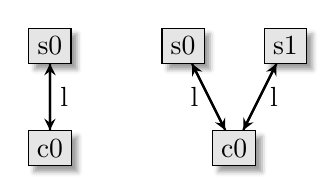
\begin{tikzpicture}[mynode/.style = {draw,inner sep=1.1mm, fill=black!10, blur shadow={shadow blur steps=3}},scale=1.3]

\node[mynode] (abar) at (0.7,0) {c0};
\node[mynode] (afoo) at (0.7,1) {s0};
\node[mynode] (bbar) at (2.5,0) {c0};
\node[mynode] (bfoo0) at (2.0,1) {s0};
\node[mynode] (bfoo1) at (3.0,1) {s1};

\begin{scope}[> = stealth,  ->,black,thick, every node/.style = {black,right,align=center}]
\draw (afoo) edge   node      {l}     (abar);
\draw (abar) edge   node      {}     (afoo);
\draw (bfoo0) edge node[left]       {l}     (bbar);
\draw (bbar) edge node       {}     (bfoo0);
\draw (bfoo1) edge   node      {l}     (bbar);
\draw (bbar) edge   node      {}     (bfoo1);
\end{scope}
\end{tikzpicture}
\end{minipage}
\\
\begin{minipage}{0.51\linewidth}
\vspace{0.05cm}
{\scriptsize
\begin{Verbatim}[commandchars=\\\{\},codes={\catcode`$=3\catcode`^=7\catcode`_=8}]
\color{blue}dtmc
\color{blue}module \color{black}c0
 x: \color{blue}bool init false\color{black};
 [r] (!x) -> 1:(x'=\color{blue}true\color{black});
\color{blue}endmodule
\color{blue}module \color{black}s0
 y: \color{blue}bool init false\color{black};
 [r] (!y) -> 0.4:(y'=\color{blue}false\color{black}) 
           + 0.6:(y'=\color{blue}true\color{black});
\color{blue}endmodule\color{black}
\end{Verbatim}
}
\end{minipage}

& 
\begin{minipage}{0.45\linewidth}
\centering
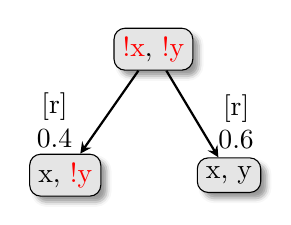
\begin{tikzpicture}[mynode/.style = {draw,inner sep=1.1mm, rounded corners, fill=black!10, blur shadow={shadow blur steps=3}},scale=1.6]
\node[mynode] (n1) at (1,1) {\red{!x}, \red{!y}};
\node[mynode] (n2) at (0.3,0) {x, \red{!y}};
\node[mynode] (n3) at (1.6,0) {x, y};
\begin{scope}[> = stealth,  ->,black,thick, every node/.style = {black,right,align=center}]
\draw (n1) edge   node[left, yshift=-1mm, xshift=-3.4mm]     {[r] \\ 0.4}     (n2);
\draw (n1) edge   node[yshift=-1mm, xshift=2mm]      {[r] \\ 0.6}     (n3);
%\draw (n2) edge [loop right] node {1.0} (n2);
%\draw (n3) edge [loop right] node {1.0} (n3);
\end{scope}
\end{tikzpicture}
\end{minipage}


\end{tabular}
\egroup
\caption{Client-server Alloy and PRISM specifications}
\label{fig:intro1}
\end{figure}

%\smallskip
%In summary, this example shows that: (i)~relational approaches lack mechanisms to reason about quantitative aspects of systems, including probabilities, (ii)~in quantitative verification, structure is fixed (including communication channels among processes), and (iii)~quantitative verification does not support systematic checking of quantitative properties across collections of design alternatives. 


\begin{figure}[!hbt]
    \centering
    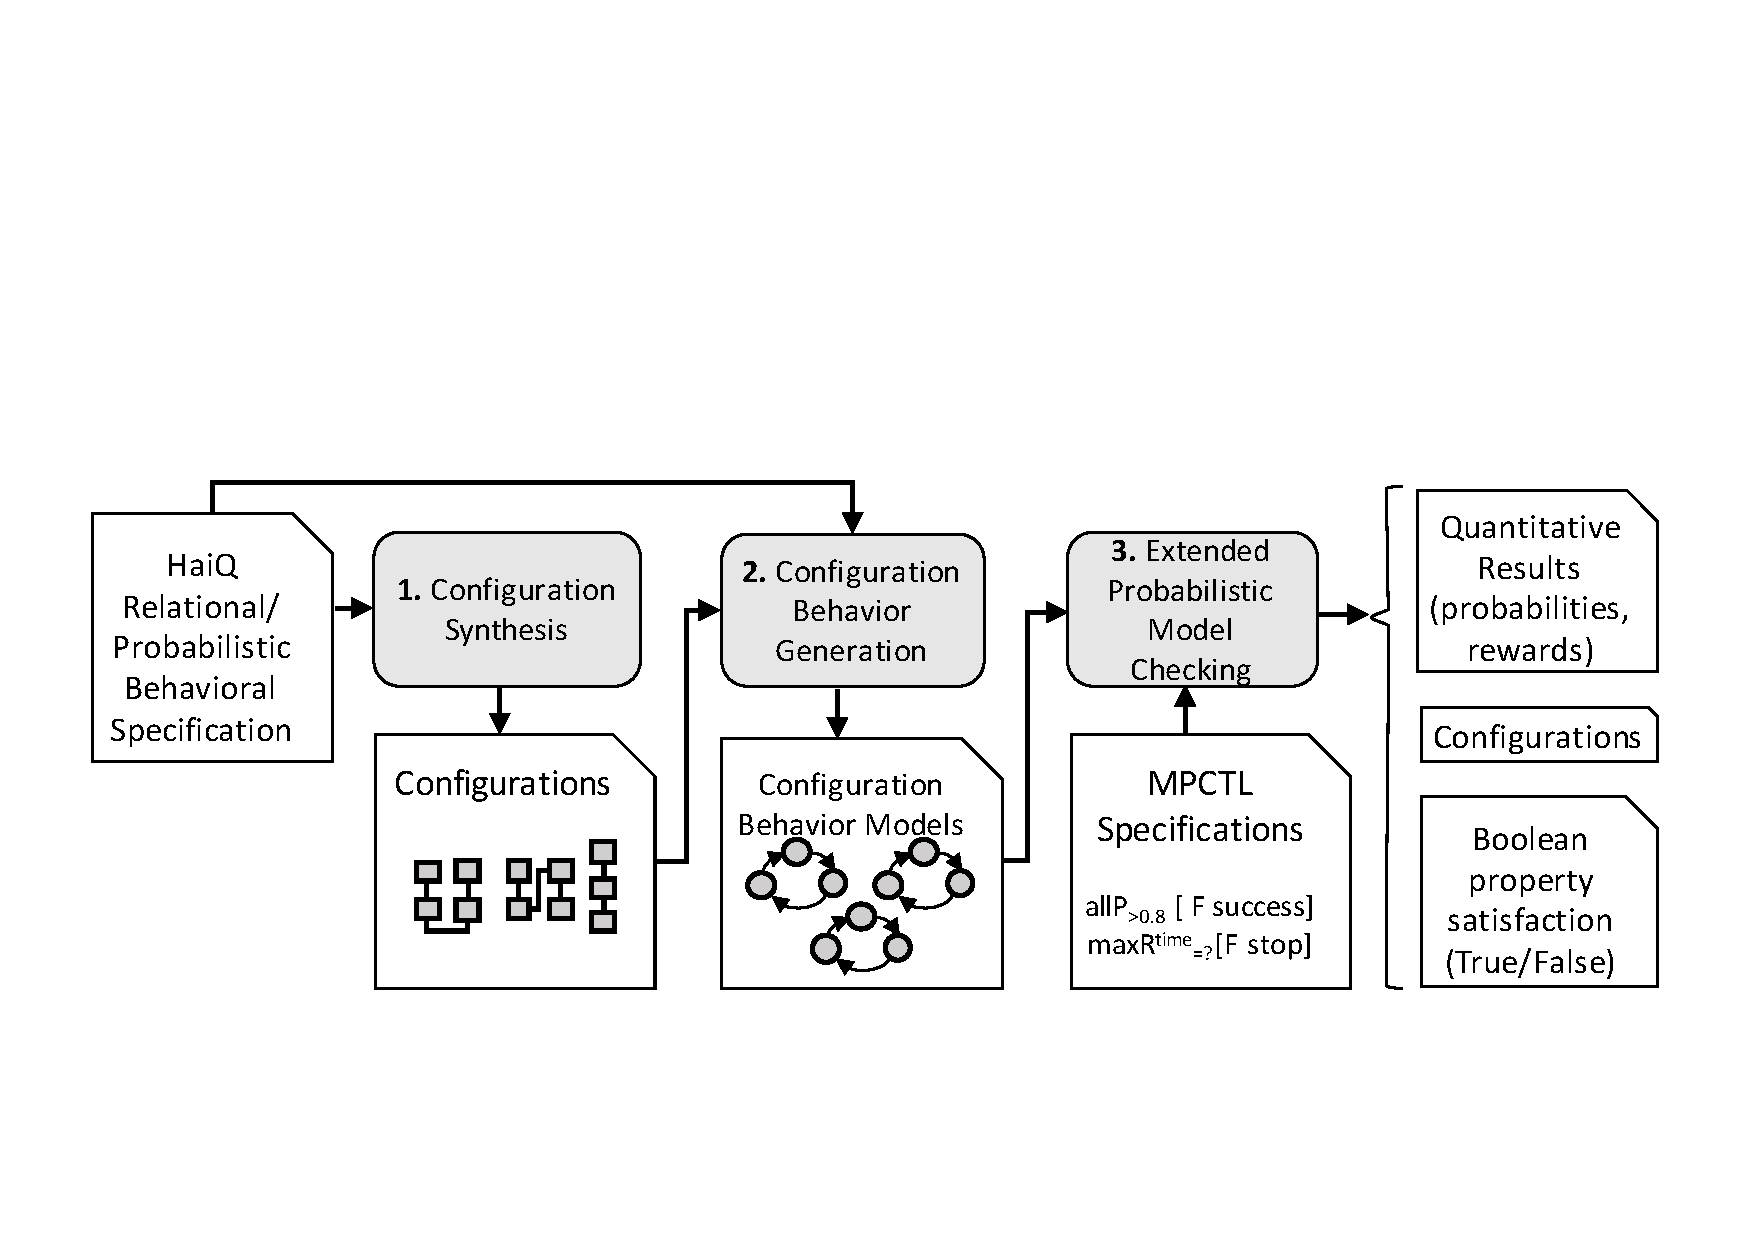
\includegraphics[width=\linewidth]{figures/overview}    
    \caption{Overview of the approach} %(adapted from~\cite{DBLP:conf/icse/WeynsC15})}
    \label{fig:overview}      
    \vspace{-0.2cm}
\end{figure}




To investigate automated joint reasoning about structural guarantees, (probabilistic) quantitative guarantees, and their interaction, our approach must: (i)~provide simple language constructs, yet expressive enough to capture structure, stochastic behavior, and their dependencies in models, (ii)~allow systematic checking of sophisticated properties on such models, and (iii)~be general enough to be applied to different domains and probabilistic analyses. 

\begin{figure*}
%\centering
\setlength{\tabcolsep}{5pt}
\begin{tabular}{c|c}
\begin{minipage}{0.28\linewidth}
{\scriptsize
\begin{Verbatim}[commandchars=\\\{\},codes={\catcode`$=3\catcode`^=7\catcode`_=8}]
\color{blue}abstract sig \color{black}comp \{l: \color{blue}some\color{black} comp\}
\color{red}</ \color{blue}var\color{black} x: \color{blue}bool init false\color{black}; 
   \color{blue}formula\color{black} p;
   [l:r] (!x) -> p : (x'=\color{blue}false\color{black}) 
             + 1-p : (x'=\color{blue}true\color{black}); \color{red}/>
\color{blue}some sig\color{black} c \color{blue}extends\color{black} comp \{\}
\color{red}</ \color{blue}formula\color{black} p=0;\color{red} />
\color{blue}some sig \color{black}s \color{blue}extends \color{black}comp \{\}
\color{red}</ \color{blue}formula \color{black}p=0.4; \color{red}/>
\color{blue}pred\color{black} clientserver \{ 
 \color{blue}disj\color{black}[c.l,c] \color{prismgreen}//only
 \color{blue}disj\color{black}[s.l,s] \color{prismgreen}//c<->s
 l = ~l \} \color{prismgreen}//symmetric relation
\color{blue}run \color{black}clientserver \color{blue}for\color{black} 1 c, 2 s
\end{Verbatim}
}
\end{minipage}
&
%\multicolumn{2}{c}{\resizebox{\linewidth}{3.8cm}{ 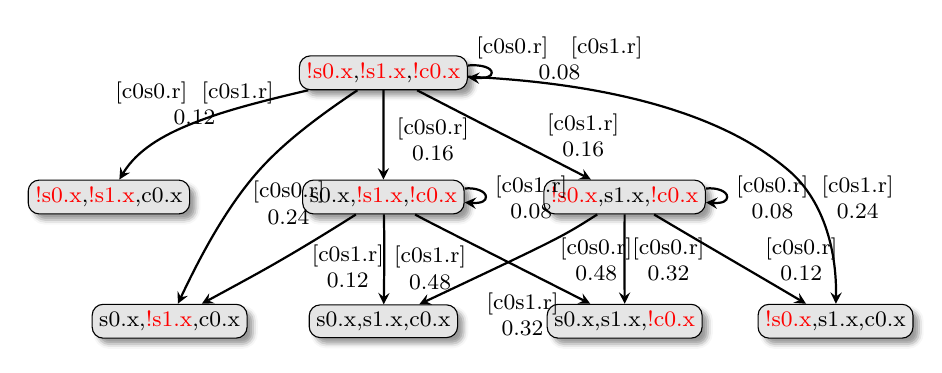
\begin{tikzpicture}[mynode/.style = {draw,inner sep=0.9mm, rounded corners, fill=black!10, blur shadow={shadow blur steps=3}},
legnode/.style = {draw,inner sep=0.9mm, fill=white, blur shadow={shadow blur steps=3}},
scale=0.52,font=\footnotesize]
%%

%\node[legnode] (leg) at (589.25bp,190.0bp) {\begin{tabular}{l} f0  = foo0 \\ f1  = foo1 \\ b0 = bar0 \\ \end{tabular}};

\node[mynode] (1) at (83.0bp,104.0bp) [draw,rectangle] {\red{!s0.x},\red{!s1.x},c0.x};
  \node[mynode] (0) at (273.0bp,190.0bp) [draw,rectangle] {\red{!s0.x},\red{!s1.x},\red{!c0.x}};
  \node[mynode] (3) at (125.0bp,18.0bp) [draw,rectangle] {s0.x,\red{!s1.x},c0.x};
  \node[mynode] (2) at (273.0bp,104.0bp) [draw,rectangle] {s0.x,\red{!s1.x},\red{!c0.x}};
  \node[mynode] (5) at (586.0bp,18.0bp) [draw,rectangle] {\red{!s0.x},s1.x,c0.x};
  \node[mynode] (4) at (440.0bp,104.0bp) [draw,rectangle] {\red{!s0.x},s1.x,\red{!c0.x}};
  \node[mynode] (7) at (273.0bp,18.0bp) [draw,rectangle] {s0.x,s1.x,c0.x};
  \node[mynode] (6) at (440.0bp,18.0bp) [draw,rectangle] {s0.x,s1.x,\red{!c0.x}};
  \begin{scope}[> = stealth,black,thick, every node/.style = {black,right,align=center}]
  \draw [->] (0) ..controls (227.66bp,159.56bp) and (203.88bp,141.62bp)  .. (186.5bp,122.0bp) .. controls (165.81bp,98.644bp) and (148.27bp,67.345bp)  .. (3);
  \draw (175.25bp,100.0bp) node {{[c0s0.r]}\\0.24};
  \draw [->] (2) ..controls (229.35bp,76.288bp) and (209.21bp,64.258bp)  .. (191.0bp,54.0bp) .. controls (183.28bp,49.652bp) and (174.99bp,45.132bp)  .. (3);
  \draw (216.25bp,56.0bp) node {{[c0s1.r]}\\0.12};
  \draw [->] (0) ..controls (273.0bp,160.26bp) and (273.0bp,145.23bp)  .. (2);
  \draw (275.25bp,144.0bp) node {{[c0s0.r]}\\0.16};
  \draw [->] (2) ..controls (336.63bp,110.65bp) and (344.0bp,108.14bp)  .. (344.0bp,104.0bp) .. controls (344.0bp,101.41bp) and (341.12bp,99.46bp)  .. (2);
  \draw (343.25bp,104.0bp) node {{[c0s1.r]}\\0.08};
  \draw [->] (4) ..controls (396.22bp,76.132bp)  .. (7);
  \draw (388.25bp,61.0bp) node {{[c0s0.r]}\\0.48};
  \draw [->] (4) ..controls (439.92bp,74.257bp) and (439.92bp,59.227bp)  .. (6);
  \draw (438.25bp,61.0bp) node {{[c0s0.r]}\\0.32};
  \draw [->] (4) ..controls (492.31bp,72.903bp) and (523.17bp,55.147bp)  .. (5);
  \draw (530.25bp,61.0bp) node {{[c0s0.r]}\\0.12};
  \draw [->] (0) ..controls (409.58bp,183.62bp) and (500.39bp,168.36bp)  .. (554.0bp,122.0bp) .. controls (576.29bp,102.72bp) and (586.93bp,69.819bp)  .. (5);
  \draw (569.25bp,104.0bp) node {{[c0s1.r]}\\0.24};
  \draw [->] (0) ..controls (333.18bp,158.73bp) and (369.07bp,140.68bp)  .. (4);
  \draw (379.25bp,147.0bp) node {{[c0s1.r]}\\0.16};
  \draw [->] (2) ..controls (273.71bp,74.257bp) and (273.71bp,59.227bp)  .. (7);
  \draw (273.25bp,55.0bp) node {{[c0s1.r]}\\0.48};
  \draw [->] (2) ..controls (301.23bp,88.412bp)  .. (6);
  \draw (337.25bp,23.0bp) node {{[c0s1.r]}\\0.32};
  \draw [->] (0) ..controls (176.7bp,167.6bp) and (156.59bp,161.39bp)  .. (138.5bp,154.0bp) .. controls (120.89bp,146.81bp) and (102.45bp,136.63bp)  .. (1);
  \draw (80.25bp,169.0bp) node {{[c0s0.r]}\; {[c0s1.r]}\\0.12};
  \draw [->] (0) ..controls (340.85bp,195.87bp) and (348.0bp,193.53bp)  .. (348.0bp,190.0bp) .. controls (348.0bp,187.74bp) and (345.07bp,185.97bp)  .. (0);
  \draw (330.25bp,200.0bp) node {{[c0s0.r]} \; {[c0s1.r]}\\0.08};
  \draw [->] (4) ..controls (503.63bp,110.65bp) and (511.0bp,108.14bp)  .. (511.0bp,104.0bp) .. controls (511.0bp,101.41bp) and (508.12bp,99.46bp)  .. (4);
  \draw (510.25bp,104.0bp) node {{[c0s0.r]}\\0.08};
 
%
\end{scope}
\end{tikzpicture}
}}
\begin{minipage}{0.72\linewidth}

\begin{tabular}{>{\centering\arraybackslash}m{0.13\linewidth} >{\centering\arraybackslash}m{0.36\linewidth} >{\centering\arraybackslash}m{0.36\linewidth}}
%\begin{tabular}{ccc}
\toprule
 & {\bf 1 client, 1 server} & {\bf 1 client, 2 servers}\\
\midrule

{\bf Structure} & 
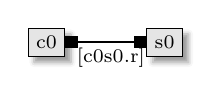
\begin{tikzpicture}[mynode/.style = {draw,inner sep=1mm, fill=black!10, blur shadow={shadow blur steps=3}},scale=1.5, font=\scriptsize]
\node[mynode] (bbar) at (0,0) {c0};
\node[mynode] (bfoo0) at (1,0) {s0};

\begin{scope}[> = stealth,  -tipSq,black,thick, every node/.style = {black,right,align=center}]
\draw (bfoo0) edge node[xshift=-5mm, yshift=-2mm]       {[c0s0.r]}     (bbar);
\draw (bbar) edge node       {}     (bfoo0);
\end{scope}
\end{tikzpicture}
& 
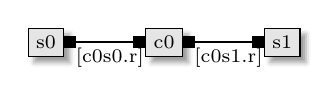
\begin{tikzpicture}[mynode/.style = {draw,inner sep=1mm, fill=black!10, blur shadow={shadow blur steps=3}},scale=1.5, font=\scriptsize]

\node[mynode] (bbar) at (1,0) {c0};
\node[mynode] (bfoo0) at (0,0) {s0};
\node[mynode] (bfoo1) at (2,0) {s1};

\begin{scope}[> = stealth,  -tipSq,black,thick, every node/.style = {black,right,align=center}]
\draw (bfoo0) edge node[xshift=-5mm, yshift=-2mm]       {[c0s0.r]}     (bbar);
\draw (bbar) edge node       {}     (bfoo0);
\draw (bfoo1) edge   node[xshift=-5mm, yshift=-2mm]      {[c0s1.r]}     (bbar);
\draw (bbar) edge   node      {}     (bfoo1);
\end{scope}
\end{tikzpicture}
\\
\midrule
{\bf State Machine} &

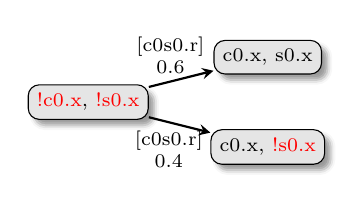
\begin{tikzpicture}[mynode/.style = {draw,inner sep=1.1mm, rounded corners, fill=black!10, blur shadow={shadow blur steps=3}},scale=1.9, font=\scriptsize]
\node[mynode] (n1) at (0,0) {\red{!c0.x}, \red{!s0.x}};
\node[mynode] (n2) at (1.2,-0.3) {c0.x, \red{!s0.x}};
\node[mynode] (n3) at (1.2,0.3) {c0.x, s0.x};
\begin{scope}[> = stealth,  ->,black,thick, every node/.style = {black,right,align=center}, every loop/.style={looseness=1}]
\draw (n1) edge   node[yshift=-3.1mm,xshift=-7mm]     {[c0s0.r] \\ 0.4}     (n2);
\draw (n1) edge   node[yshift=3mm,xshift=-7mm]      {[c0s0.r] \\ 0.6}     (n3);
%\draw (n2) edge [loop right] node {1.0} (n2);
%\draw (n3) edge [loop right] node {1.0} (n3);
\end{scope}
\end{tikzpicture}

& 

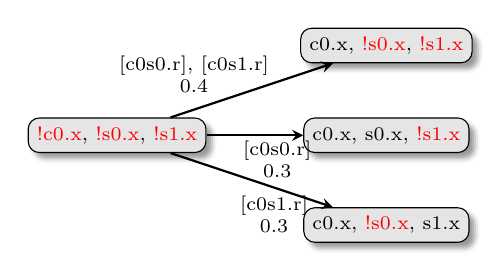
\begin{tikzpicture}[mynode/.style = {draw,inner sep=1.1mm, rounded corners, fill=black!10, blur shadow={shadow blur steps=3}},scale=1.9, font=\scriptsize]
\node[mynode] (n1) at (0,0) {\red{!c0.x}, \red{!s0.x}, \red{!s1.x}};
\node[mynode] (n2) at (1.8,0.6) {c0.x, \red{!s0.x}, \red{!s1.x}};
\node[mynode] (n3) at (1.8,0) {c0.x, s0.x, \red{!s1.x}};
\node[mynode] (n4) at (1.8,-0.6) {c0.x, \red{!s0.x}, s1.x};
\begin{scope}[> = stealth,  ->,black,thick, every node/.style = {black,right,align=center}, every loop/.style={looseness=1}]
\draw (n1) edge   node[yshift=-3mm, xshift=-2.8mm]      {[c0s0.r] \\ 0.3}     (n3);
\draw (n1) edge   node[yshift=-4.3mm, xshift=-2.8mm]      {[c0s1.r] \\ 0.3}     (n4);
\draw (n1) edge   node[left, yshift=2mm, xshift=3.5mm]     {[c0s0.r], [c0s1.r] \\ 0.4}     (n2);
%\draw (n2) edge [loop right] node {1.0} (n2);
%\draw (n3) edge [loop right] node {1.0} (n3);
%\draw (n4) edge [loop right] node {1.0} (n4);
\end{scope}
\end{tikzpicture}
\\

\bottomrule

\end{tabular}

\end{minipage}
\end{tabular}

\caption{Client-server {\sf HaiQ} specification (left), implicit structure collection and corresponding state machines (right)}
\label{fig:intro2}
\end{figure*}


To address these requirements, we propose an approach that includes: (i)~a high-level language ({\sf HaiQ}) for modeling collections of probabilistic models as {\em relational/probabilistic behavioral specifications}, and (ii)~a language for specifying (and associated mechanisms for checking) quantitative temporal properties (probability- and reward-based) on collections of probabilistic models ({\em manifold probabilistic computation tree logic} or M-PCTL).


We embody these languages and reasoning mechanisms in a relational probabilistic model checker that combines synthesis of structural designs from relational constraints, with model checking of individual designs obtained from the structural specification of synthesized design variants (Figure~\ref{fig:overview}). 
Our proposal includes three consecutive stages:
{\bf (i)~Configuration Synthesis}, during which topological descriptions of configurations are synthesized from the relational constraints of a {\sf HaiQ} model,
{\bf (ii)~Configuration Behavioral Model Generation}, which uses configuration descriptions synthesized in the previous stage as a blueprint to generate a full-blown probabilistic behavioral model for every configuration (supported model types are DTMC and MDP),
{\bf (iii)~Extended Probabilistic Model Checking}, which uses as input properties specified in M-PCTL to provide quantitative results about the set of configuration behavioral models generated. Supported analyses include average probability-based and reward-based guarantees for DTMC and worst/best case probability-based and reward-based guarantees for MDP.



%The approach consists of two main elements: (i)~a high-level language for modeling collections of probabilistic models (discrete-time Markov Chains or DTMC), and (ii)~a language for checking quantitative temporal properties (probability- and reward-based) on collections of probabilistic models.
\smallskip
\noindent {\bf The {\sf HaiQ} Modeling Language.} 
{\sf HaiQ} specifications juxtapose static (or structural) relational descriptions with blocks of probabilistic behavioral specification that can exploit the information about system structure encoded in relations. 

To illustrate the main ideas behind the language, we focus on a simple {\sf HaiQ} specification that builds on our introductory example (Figure~\ref{fig:intro2}). Here, the possible structures of the system are similar to the ones captured by the Alloy specification in Figure~\ref{fig:intro1}. 
In contrast with Alloy, {\sf HaiQ} signatures include blocks of behavior specifications (between ``{\tt</}'' and ``{\tt/>}'') that enclose guarded probabilistic commands. 
This is because {\it every signature in {\sf HaiQ} is also a process type}. 
Let us emphasize that, in contrast with the languages employed by existing probabilistic model checkers, {\em behavioral descriptions in {\sf HaiQ} are at a higher level of abstraction and denote process types, not process instances}. 
This means that {\it a {\sf HaiQ} model implicitly describes a process type hierarchy associated with signatures in which behaviors can be inherited and extended}. 
In the example, this can be observed in the command included in signature {\tt comp}, which is defined in a generic manner and inherited by signatures {\tt c} and {\tt s}. 
In particular, the synchronization action {\tt r} in the command is prefixed by the relation {\tt l} defined in the static part of the specification, indicating that the {\it synchronization matches only processes that correspond to signature instances in the relation (independently of the topology under which they are instantiated), rather than being ``hardwired''} as we saw in the PRISM example in Figure~\ref{fig:intro1}. 
The top-right of Figure~\ref{fig:intro2} shows the two possible structure instantiations of the specification, in which process instances {\tt s0} and {\tt s1} synchronize with {\tt c0} on actions generated based on the instantiation of relation {\tt l}. 
The corresponding probabilistic state machines that result from the parallel composition of the behaviors of the {\tt c-s} instances are shown in the right-bottom.

The details of the modeling language are described in Section~\ref{sec:haiq}.

\smallskip
\noindent {\bf Manifold Probabilistic Computation Tree Logic (M-PCTL)}. 
Ultimately, a {\sf HaiQ} model defines a set of probabilistic state machines (DTMC or MDP), where each one of them results from the parallel composition of processes instantiated in accordance with each topology that satisfies the model's structural constraints. 
Formulas in existing probabilistic temporal logics like PCTL capture properties of a single probabilistic state machine. 
Hence, our work extends existing languages to query {\sf HaiQ} specifications and {\it check properties across entire collections of probabilistic state machines}, rather than individual instances. 
M-PCTL is an extension of PCTL including new operators and quantifiers that enable designers to check properties like ``across all configurations, the minimum probability that a service will never time out is greater than 0.95'', and ``there exists a robot configuration that requires less than 3.2 whr to achieve its goal.''

In our client-server example, the property ${\sf allP_{\geq 0.6} [ F \; all \; c.x \wedge some \; s.x]}$ can be interpreted as ``for all configurations, the probability that all requests will be correctly sent by the client and at least one of them will be correctly received by a server is at least 0.6'' 
In this case, the property check returns true, because for the two possible configurations (with one and two servers), the probabily that ${\sf [F \; all \; c.x \wedge some \; s.x]}$ is satisfied is exactly 0.6 in both cases.
Moreover, {\it M-PCTL properties can also return structures that optimize or satisfy some quantitative property}. 
For instance, the property ${\sf SmaxP\; [ F \; all \; c.x \wedge some \; s.x]}$ returns a set including a description of the one-server and the two-server configurations, since both of them have the same probability of satisfying ${\sf [F \; all \; c.x \wedge some \; s.x]}$ and hence maximize the value of the property in this case because there are no other feasible solutions. 

% \smallskip
% In our client-server example, ${\sf SmaxPmin [ F \; all \; c.x \wedge some \; s.x]}$ is a property that can be interpreted as ``for all configurations, the probability that all requests will be correctly sent by the client and at least one of them will be correctly received by a server is at least 0.6'' 
% In this case, the property check returns true, because for the two possible configurations (with one and two servers), the probabily that ${\sf [F \; all \; c.x \wedge some \; s.x]}$ is satisfied is exactly 0.6 in both cases.
% Moreover, {\it M-PCTL properties can also return structures that optimize or satisfy some quantitative property}. 
% For instance, the property ${\sf SmaxP\; [ F \; all \; c.x \wedge some \; s.x]}$ returns a description of the two-server configuration, which is the one that maximizes the probability of satisfying ${\sf [F \; all \; c.x \wedge some \; s.x]}$. 



% Following with the example shown in Figure~\ref{fig:intro2}, the property ${\sf allP_{\geq 0.8} [ F \; all \; foo.x=true]}$ can be interpreted as ``across all configurations, the probability that variable {\tt x} will eventually be true in all {\tt foo} instances is always greater or equal to 0.8.'' 
% In this case, the property check returns false, because for the two possible configurations (with one and two {\tt foo} instances), the probabilities that all {\tt foo.x} are eventually true are 0.869 and 0.302, respectively. 
% Moreover, {\bf M-PCTL properties can also return structures that optimize or satisfy some quantitative property}. 
% For instance, the property ${\sf SminP\; [ F \; all \; foo.x=true]}$ returns a description of the structure with two {\tt foo} instances, which is the one that minimizes the probability of satisfying ${\sf [ F \; all \; foo.x=true]}$. 


The syntax and semantics of M-PCTL are described in Section~\ref{sec:mpctl}.

\section{The {\sf HaiQ} Modeling Language}
\label{sec:haiq}

In this section, we formalize the modeling language and illustrate its main features by modeling a simple network security scenario introduced by Kwiatkowska et al~\cite{KNPV09}.\footnote{A PRISM model for this network security scenario can be found in http://www.prismmodelchecker.org/casestudies/virus.php.} 
The scenario models the progression of a virus infecting a network formed by a grid of N$\times$N nodes. 
The virus remains at a node that is infected and repeatedly tries to infect any uninfected neighbors by first attacking the neighbor's firewall and, if successful, trying to infect the node.

In the network there are 'low' and 'high' nodes divided by 'barrier' nodes that scan the traffic between them. 
Initially, only one corner 'low' node is infected. A graphical representation of the network when N=3 is given in Figure~\ref{fig:virusscenario}.

% Virus network spread

\begin{figure}[]

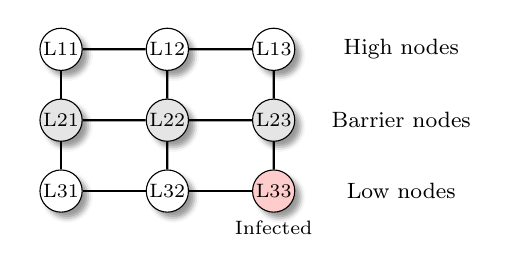
\begin{tikzpicture}[scale=0.6,
 locnode/.style = {draw,inner sep=0.2mm, circle,fill=white, blur shadow={shadow blur steps=3}},
 ilocnode/.style = {draw,inner sep=0.2mm, circle,fill=red!20, blur shadow={shadow blur steps=3}},
 blocnode/.style = {draw,inner sep=0.2mm, circle,fill=black!10, blur shadow={shadow blur steps=3}},
 scale=1.5]


\node[locnode] (L31) at (0,0) {\scriptsize L31};
\node[locnode] (L32) at (1.5,0) {\scriptsize L32};
\node[ilocnode] (L33) at (3,0) {\scriptsize L33};
\node (LNL) at (4.8,0) {\footnotesize Low nodes};

\node[blocnode] (L21) at (0,1) {\scriptsize L21};
\node[blocnode] (L22) at (1.5,1) {\scriptsize L22};
\node[blocnode] (L23) at (3,1) {\scriptsize L23};
\node (BNL) at (4.8,1) {\footnotesize Barrier nodes};

\node[locnode] (L11) at (0,2) {\scriptsize L11};
\node[locnode] (L12) at (1.5,2) {\scriptsize L12};
\node[locnode] (L13) at (3,2) {\scriptsize L13};
\node (HNL) at (4.8,2) {\footnotesize High nodes};

\node (inf) at (3,-0.52) {\scriptsize Infected};


\begin{scope}[> = stealth,  -,black,thick, every node/.style = {black,right,align=center}]
% Horizontal
\draw (L11) edge node[left, xshift=-5pt]       {}     (L12);
\draw (L12) edge node[left, xshift=-5pt]       {}     (L13);

\draw (L21) edge node[left, xshift=-5pt]       {}     (L22);
\draw (L22) edge node[left, xshift=-5pt]       {}     (L23);

\draw (L31) edge node[left, xshift=-5pt]       {}     (L32);
\draw (L32) edge node[left, xshift=-5pt]       {}     (L33);

% Vertical
\draw (L11) edge node[left, xshift=-5pt]       {}     (L21);
\draw (L21) edge node[left, xshift=-5pt]       {}     (L31);

\draw (L12) edge node[left, xshift=-5pt]       {}     (L22);
\draw (L22) edge node[left, xshift=-5pt]       {}     (L32);

\draw (L13) edge node[left, xshift=-5pt]       {}     (L23);
\draw (L23) edge node[left, xshift=-5pt]       {}     (L33);


\end{scope}
\end{tikzpicture}
%\vspace{-0.3cm}
\caption{Network virus infection scenario}
\label{fig:virusscenario}
%\vspace{-0.5cm}
\end{figure}

\subsection{Language Features}

\subsubsection{Signatures as Structural and Behavioral Building Blocks}
The modeling language is tailored for the incremental construction of structured probabilistic models. 
The basic unit of specification is the {\em signature}, which contains structural and behavioral code fragments. 
The structural part of the language is a subset of the static part of Alloy (c.f.~\cite{DBLP:books/daglib/0024034}, 2.1), in which every signature field is a set that defines implicitly a binary relation between the instances of signatures in which the field is declared and the elements in the set.\footnote{{\sf HaiQ}'s grammar is described in the supplement submitted with this paper.} For example, the field {\tt conn} declared in the first line of the {\tt node} definiton listing encodes a relation capturing the fact that a node can be connected to one or more neighboring nodes (i.e., {\tt conn} is implicitly encoding the arcs in the network graph shown in Figure~\ref{fig:virusscenario}). Constraining fields of signatures to this type of relation suffices to capture sophisticated topologies and limits the complexity of specifications. 
Note that the declaration states that signature {\tt node} is {\em abstract}, so it can be extended by other signatures:

%We start to build incrementally the model for the scenario declaring a signature {\tt node} that captures the locations in the network:

%\smallskip
%\noindent\rule[0.5ex]{\linewidth}{1pt}
{\scriptsize
\begin{Verbatim}[commandchars=\\\{\},codes={\catcode`$=3\catcode`^=7\catcode`_=8}]
\color{blue}abstract sig \color{black}node \{conn: \color{blue}some \color{black}node\}
\color{red}</ \color{blue}enum \color{black}modes:\{uninfected, breached, infected\};
   \color{blue}var \color{black}s:[modes] \color{blue}init \color{black}uninfected;
   \color{blue}formula \color{black}detect=node\_detect;
   \color{black}[conn:attack] (s=uninfected) -> 1-detect : (s'=breached)
    \color{prismgreen}/* firewall attacked */       \color{black} + detect : (s'=s);
   \color{black}[] (s=breached) ->  1-infect : (s'=uninfected)
                      \color{black} + infect : (s'=infected);
   [conn:attack] (s=infected) -> \color{blue}true; \color{red}/>
\end{Verbatim}
}

%\noindent\rule[0.5ex]{\linewidth}{1pt}
%\smallskip
The second part of the signature encodes its behavior and is surrounded by the process block delimiters ``{\tt</}'' and ``{\tt />}''. 
Process blocks include a set of local variables that can be bounded integers~\footnote{For convenience, the language also provides enumerated types, which are internally treated as integer variables.} or booleans, as well as formulas that are used as shorthand for complex expressions to avoid code duplications. 
In the example, variable {\tt s} specifies the state of the node ({\tt uninfected}, {\tt breached}, {\tt infected}), and formula {\tt detect} encodes the probability that the virus is detected by the firewall in the node. 
Constants {\tt node\_detect} and {\tt infect} are global constants that encode a default probability value for firewall detection and node infection. % The formula in this case is underspecified because it will be overriden by other non-abstract signatures extending {\tt node}, discussed later in this section. 

Finally, the process block includes a set of probabilistic guarded commands that describe the behavior of the signature. 
Each command describes the possible transitions of the process in states that satisfy its guard (specified before {``{\tt->}''}), and a set of updates that specify each one of the possible outcomes as sets of new values for (primed or post-) state variables (e.g., {\tt s'=infected}). 
Each update is associated with a probability, and unspecified state variables in an update indicate no change in value. 
In the first command of the example, the guard specifies that when the node is not infected, it can be attacked with two possible outcomes. With probability {\tt detect}, the firewall will remain unbreached, and with probability 1-{\tt detect}, the firewall will be successfully breached by the attack. 

Note that the prefixing of the action by {\tt conn} indicates that the behavior specified by this command is replicated for each of the {\tt node} instances in the relation. 
Hence, for an example system structure with a node instance {\tt A} in which {\tt A.conn=\{B,C\}}, each command in the process block labeled as {\tt [conn:attack]} is denoting two alternative actions {\tt [A.B.attack]} and {\tt[A.C.attack]}\footnote{The syntax of these labels is used only for illustration purposes. Internally, the {\sf HaiQ} compiler generates a unique identifier using a commutative function (the identifier for inputs (A,B) is the same as for (B,A)), resulting in a label that can be employed on both endpoints of process synchronization (c.f. Section~\ref{sec:csbm}).} that can synchronize with actions of the same name in nodes {\tt B} and {\tt C}.

\subsubsection{Synchronization}

% Synchronization scheme for two sample node instances
\begin{figure}[]
 \resizebox{.99\linewidth}{!}{
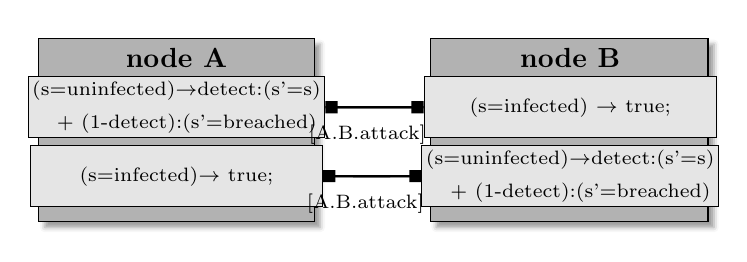
\begin{tikzpicture}[mynode/.style = {draw,inner sep=0.5mm, fill=black!10},scale=2.5, 
                     minimum height={22pt}, minimum width={width(" (s=uninfected) -> detec")}]

\filldraw[fill=black!30!white, draw=black,blur shadow={shadow blur steps=3}] (-0.7,0.92) rectangle (0.7,1.85);
\node (A) at (0, 1.75) {\textbf{node A}};

\filldraw[fill=black!30!white, draw=black,blur shadow={shadow blur steps=3}] (1.289,0.92) rectangle (2.7,1.85);
\node (B) at (2, 1.75) {\textbf{node B}};

\node[mynode] (A1) at (0,1.15) {\scriptsize (s=infected)$\rightarrow$ true;};
\node[mynode] (B1) at (2,1.15) [align=left]{\scriptsize (s=uninfected)$\rightarrow$detect:(s'=s)\\ \;\; \scriptsize + (1-detect):(s'=breached)};

\node[mynode] (A2) at (0,1.5) [align=left]{\scriptsize (s=uninfected)$\rightarrow$detect:(s'=s)\\ \;\; \scriptsize + (1-detect):(s'=breached)};
\node[mynode] (B2) at (2,1.5) {\scriptsize (s=infected) $\rightarrow$ true;};

\begin{scope}[> = stealth,  -tipSq,black,thick, every node/.style = {black,right,align=center}]
\draw (A1) edge node[left,xshift=46pt,yshift=-10pt]       {\scriptsize \;\;\; [A.B.attack]}     (B1);
\draw (B1) edge node                                      {}                 (A1);

\draw (A2) edge node[left,xshift=46pt,yshift=-10pt]       {\scriptsize \;\;\; [A.B.attack]}     (B2);
\draw (B2) edge node                                      {}                 (A2);

\end{scope}
\end{tikzpicture}
}
\caption{Sample synchronization scheme between nodes}
\label{fig:synch}
\end{figure}

Different signature processes in a specification synchronize on shared action names. 
The third command of the {\tt node} behavior definition contains an action labeled {\tt attack} prefixed by {\tt conn}, just like in the first command that we saw earlier. 
In this case, the command models the transition in which the infected node attacks a neighboring node with probability 1 (unspecified probability in a command defaults to 1). 
Consider an example of two neighbor node instances {\tt A} and {\tt B}, in which {\tt A.conn=\{B\}} and {\tt B.conn=\{A\}} (Figure~\ref{fig:synch}). 
In the scheme, nodes synchronize on the same action name {\tt [A.B.attack]} both when the node attacks and receives an attack from a neighboring node. 
However, the commands synchronize pairwise because the guards in commands on the same module are mutually exclusive. 
Hence, whenever node {\tt A} attacks, node {\tt B} receives the attack, and vice versa.

\subsubsection{Subtyping and Extension}

Signatures can be extended to incorporate new structural and behavioral elements. 
Similarly to Alloy, a signature that extends another one is considered its subtype. 
However, in this case subtyping also implies inheritance not only of the structural elements of the extended signature, but also of its behavioral definition.
The following listing encodes the subtypes of node for the network scenario:

%\smallskip
%\noindent\rule[0.5ex]{\linewidth}{1pt}
{\scriptsize
\begin{Verbatim}[commandchars=\\\{\},codes={\catcode`$=3\catcode`^=7\catcode`_=8}]
\color{blue}sig \color{black}barrierNode \color{blue}extends \color{black}node \{\} 
 \color{red}</ \color{blue}formula \color{black}detect=barrier\_detect; \color{red}/>
\color{blue}sig \color{black}highNode, lowNode \color{blue}extends \color{black}node \{\}
\color{blue}one sig \color{black}infectedNode \color{blue}extends \color{black}lowNode \{\} 
 \color{red}</ \color{blue}var \color{black}s:[modes] \color{blue}init \color{black}infected; \color{red}/>
\end{Verbatim}
}

%\noindent\rule[0.5ex]{\linewidth}{1pt}
First, signature {\tt barrierNode} extends signature {\tt node} to create a special type of node in which the attack detection probability is different to the rest of the nodes (encoded in constant {\tt barrier\_detect}). This is achieved by overriding the original definition of the formula {\tt detect} in the abstract signature {\tt node}.

In contrast, {\tt highNode} and {\tt lowNode} are subtypes of {\tt node} that preserve all its structural and behavioral elements intact because we are only interested in formally distinguishing them as special locations, but do not require to incorporate any special behaviors.

Finally, we incorporate {\tt infectedNode} as a subtype of {\tt lowNode} to include an infected node in the scenario. This type is constrained to a singleton (keyword {\tt one}) and overrides the declaration of the node state variable, which is now initialized as {\tt infected}.

\subsubsection{Topology}

The possible topologies of design alternatives that can be generated by a {\sf HaiQ} model are defined implicitly by a set of structural constraints expressed in relational logic sentences. 

\smallskip
%\noindent\rule[0.5ex]{\linewidth}{1pt}
{\scriptsize
\begin{Verbatim}[commandchars=\\\{\},codes={\catcode`$=3\catcode`^=7\catcode`_=8}]
pred virus\{ \color{blue}all \color{black}n:node | node \color{blue}in \color{black}n.*conn \color{prismgreen}// connected network
  (\color{blue}no iden \color{black}& conn) \color{blue}and \color{black}(conn=~conn) \color{prismgreen}//no self-loops, symmetry
  \color{blue}disj\color{black}[lowNode.conn,highNode] \} \color{prismgreen}//disjoint low-high nodes
\end{Verbatim}
}
% \color{blue}all \color{black}n,n':node | (n' \color{blue}in \color{black}n.\string^conn \color{blue}and \color{blue}disj\color{black}[n,n.conn]) \color{blue}and
%   \color{blue}all \color{black}b:barrierNode | \color{blue}not disj\color{black}[highNode+lowNode, b.conn] \color{blue}and
%   \color{blue}all \color{black}n:node | #n.conn & barrierNode <=1 \color{blue}and
%   \color{blue}all \color{black}n:lowNode | #n.conn & lowNode <=2 \color{blue}and
%   \color{blue}all \color{black}n:highNode | #n.conn & highNode <=2 \color{blue}and
%   \color{blue}disj\color{black}[lowNode.conn,highNode] \color{blue}and
%   \color{blue}all \color{black}n,n':node | n \color{blue}in \color{black}n'.conn <=> n' \color{blue}in \color{black}n.conn \}

In the example, the first constraint imposes that all nodes must be reachable in the network from any other node. 
The second constraint specifies that connections are symmetric and that no node must be connected to itself, whereas the third one imposes that low nodes and high nodes must never be directly connected. 
Figure~\ref{fig:virusconfigs} shows two of the many legal configurations that can be synthesized from the virus infection scenario model (apart from the one shown in Figure~\ref{fig:virusscenario}) for a scope of {\tt N=3} by running: {\footnotesize \tt \color{blue}run \color{black}virus \color{blue}for exactly \color{black}3 lowNode, \color{blue}exactly \color{black}3 barrierNode, \color{blue}exactly \color{black}3 highNode}.

%\noindent\rule[0.5ex]{\linewidth}{1pt}
%{\footnotesize
%\begin{Verbatim}[commandchars=\\\{\},codes={\catcode`$=3\catcode`^=7\catcode`_=8}]
%\color{blue}run \color{black}virus 3 lowNode, 3 barrierNode, 3 highNode
%\end{Verbatim}
%}
% Virus network infection configurations

\begin{figure}[t]
\def\oc{5}
\begin{tikzpicture}[scale=0.4,
 locnode/.style = {draw,inner sep=0.15mm, circle,fill=white, blur shadow={shadow blur steps=3}},
 ilocnode/.style = {draw,inner sep=0.15mm, circle,fill=red!20, blur shadow={shadow blur steps=3}},
 blocnode/.style = {draw,inner sep=0.15mm, circle,fill=black!10, blur shadow={shadow blur steps=3}},
 scale=1.8]



\node[locnode] (alowNode0) at (0+\oc,0) {\scriptsize L31};
\node[locnode] (alowNode1) at (1.5+\oc,0) {\scriptsize L32};
\node[ilocnode] (ainfectedNode0) at (3+\oc,0) {\scriptsize L33};

\node[blocnode] (abarrierNode2) at (0+\oc,1) {\scriptsize L21};
\node[blocnode] (abarrierNode1) at (1.5+\oc,1) {\scriptsize L22};
\node[blocnode] (abarrierNode0) at (3+\oc,1) {\scriptsize L23};

\node[locnode] (ahighNode0) at (0+\oc,2) {\scriptsize L11};
\node[locnode] (ahighNode1) at (1.5+\oc,2) {\scriptsize L12};
\node[locnode] (ahighNode2) at (3+\oc,2) {\scriptsize L13};


\node[locnode] (lowNode0) at (0,0) {\scriptsize L31};
\node[locnode] (lowNode1) at (1.5,0) {\scriptsize L32};
\node[ilocnode] (infectedNode0) at (3,0) {\scriptsize L33};
%\node (LNL) at (4,0) {Low nodes};

\node[blocnode] (barrierNode2) at (0,1) {\scriptsize L21};
\node[blocnode] (barrierNode1) at (1.5,1) {\scriptsize L22};
\node[blocnode] (barrierNode0) at (3,1) {\scriptsize L23};
%\node (BNL) at (4,1) {Barrier nodes};

\node[locnode] (highNode0) at (0,2) {\scriptsize L11};
\node[locnode] (highNode1) at (1.5,2) {\scriptsize L12};
\node[locnode] (highNode2) at (3,2) {\scriptsize L13};
%\node (HNL) at (4,2) {High nodes};



\begin{scope}[> = stealth,  -,black,thick, every node/.style = {black,right,align=center}]
\draw (lowNode1) edge [left]   node     {}     (infectedNode0);
\draw (highNode2) edge [left]   node     {}     (barrierNode0);
\draw (lowNode1) edge [left]   node     {}     (lowNode0);
\draw (highNode1) edge [left]   node     {}     (barrierNode1);
\draw (barrierNode2) edge [left]   node     {}     (highNode0);
\draw (lowNode0) edge [left]   node     {}     (lowNode1);
\draw (infectedNode0) edge [left]   node     {}     (lowNode1);
\draw (lowNode0) edge [left]   node     {}     (barrierNode2);
\draw (barrierNode1) edge [left]   node     {}     (lowNode1);
\draw (barrierNode2) edge [left]   node     {}     (lowNode0);
\draw (infectedNode0) edge [left]   node     {}     (barrierNode0);
\draw (barrierNode1) edge [left]   node     {}     (barrierNode2);
%\draw (lowNode0) edge [bend right]   node     {}     (infectedNode0);
\draw (barrierNode2) edge [left]   node     {}     (barrierNode1);
\draw (lowNode1) edge [left]   node     {}     (barrierNode1);
\draw (barrierNode0) edge [left]   node     {}     (highNode2);
\draw (highNode0) edge [left]   node     {}     (barrierNode2);
\draw (barrierNode1) edge [left]   node     {}     (highNode1);
\draw (barrierNode0) edge [left]   node     {}     (infectedNode0);


% \draw (lowNode1) edge [left]   node     {}     (lowNode0);
% \draw (highNode1) edge [left]   node     {}     (barrierNode2);
% \draw (infectedNode0) edge [left]   node     {}     (lowNode0);
% \draw (barrierNode0) edge [left]   node     {}     (barrierNode1);
% \draw (barrierNode0) edge [bend right]   node     {}     (barrierNode2);
% \draw (barrierNode2) edge [left]   node     {}     (lowNode0);
% \draw (barrierNode0) edge [left]   node     {}     (lowNode1);
% \draw (lowNode0) edge [left]   node     {}     (infectedNode0);
% \draw (barrierNode2) edge [left]   node     {}     (barrierNode1);
% \draw (lowNode1) edge [left]   node     {}     (barrierNode1);
% \draw (lowNode1) edge [left]   node     {}     (barrierNode0);
% \draw (barrierNode2) edge [left]   node     {}     (infectedNode0);
% \draw (barrierNode2) edge [left]   node     {}     (highNode0);
% \draw (highNode2) edge [left]   node     {}     (barrierNode1);
% \draw (lowNode0) edge [left]   node     {}     (lowNode1);
% \draw (infectedNode0) edge [left]   node     {}     (barrierNode2);
% \draw (lowNode0) edge [left]   node     {}     (barrierNode2);
% \draw (barrierNode2) edge [left]   node     {}     (highNode1);
% \draw (barrierNode1) edge [left]   node     {}     (lowNode1);
% \draw (infectedNode0) edge [left]   node     {}     (barrierNode0);
% \draw (barrierNode1) edge [left]   node     {}     (barrierNode2);
% \draw (barrierNode1) edge [left]   node     {}     (barrierNode0);
% \draw (highNode0) edge [left]   node     {}     (barrierNode2);
% \draw (barrierNode1) edge [left]   node     {}     (highNode2);
% \draw (barrierNode0) edge [left]   node     {}     (infectedNode0);

\draw (ahighNode2) edge [left]   node     {}     (abarrierNode0);
\draw (ahighNode1) edge [left]   node     {}     (abarrierNode1);
\draw (abarrierNode2) edge [left]   node     {}     (ahighNode0);
\draw (alowNode0) edge [left]   node     {}     (abarrierNode2);
\draw (abarrierNode1) edge [left]   node     {}     (alowNode1);
%\draw (ahighNode2) edge [bend right]   node     {}     (ahighNode0);
\draw (ahighNode2) edge [left]   node     {}     (ahighNode1);
\draw (abarrierNode2) edge [left]   node     {}     (alowNode0);
\draw (ahighNode0) edge [left]   node     {}     (ahighNode1);
\draw (ainfectedNode0) edge [left]   node     {}     (abarrierNode0);
\draw (alowNode1) edge [left]   node     {}     (abarrierNode1);
\draw (abarrierNode0) edge [left]   node     {}     (ahighNode2);
\draw (ahighNode0) edge [left]   node     {}     (abarrierNode2);
\draw (ahighNode1) edge [left]   node     {}     (ahighNode2);
\draw (abarrierNode1) edge [left]   node     {}     (ahighNode1);
\draw (abarrierNode0) edge [left]   node     {}     (ainfectedNode0);
\draw (ahighNode1) edge [left]   node     {}     (ahighNode0);



\end{scope}
\end{tikzpicture}

\caption{Alternative legal network configurations}
\label{fig:virusconfigs}
\end{figure}
\subsubsection{Rewards}
{\sf HaiQ} can be used to reason, not just about the probability that a collection of behaviors specified by a model behaves in a certain fashion, but about a wider range of quantitative measures relating to behaviour. 
This includes properties such as ``expected time'' or ``expected power consumption.'' 

This is achieved by augmenting signatures with rewards, which are real values associated with certain model states or transitions. 
We include in our example a reward that enables us to quantify the number of attack attempts carried out by the different nodes:

%\noindent\rule[0.5ex]{\linewidth}{1pt}
{\scriptsize
\begin{Verbatim}[commandchars=\\\{\},codes={\catcode`$=3\catcode`^=7\catcode`_=8}]
\color{blue}abstract sig \color{black}node \{conn: \color{blue}some \color{black}node\}
\color{red}</ \color{black}... \color{blue}reward \color{black}attacks [conn:attack]  \color{blue}true\color{black} : 1; \color{red}/>
\end{Verbatim}
}

The reward is associated with transitions in which the action {\tt attack} is executed from any state. 
Every time the action is executed from a state in which the guard before the colon is satisfied (in this case, the guard is {\tt true} and is therefore always satisfied), a reward of one unit will be accrued for {\tt attacks}.
The prefixing of the action by relation {\tt conn} results in reward cumulation for any of the instances of the action executed among any arbitrary pair of nodes.

\subsection{Formal Model}
\label{subsec:formalmodel}




% \medskip
% %{\footnotesize
% \begin{tabbing}
% sigDecl ::= \= [mult] {\bf sig} sigID [{\bf extends} sigID] sigBody\\
% sigBody ::= \= sigStatic sigProcess\\
% sigStatic ::= \= {\bf \{} declSetExpr, \textsuperscript{*} {\bf \}} [constraintSeq] \\
% declSetExpr ::=  \= [{\bf part} | {\bf disj}] varId,\textsuperscript{+} {\bf :} [mult] sigId \\
% mult ::= \= {\bf lone} | {\bf one} | {\bf some}\\
% constraintSeq ::= {\bf \{} constraint \textsuperscript{*} {\bf \}}\\
% constraint ::= \= expr [{\bf not}] compOp expr \\
%                 \> | quantifier expr\\
%                 \> | {\bf not} constraint | constraint logicOp constraint\\
%                 \> | constraint {\bf =>} constraint\\
%                 \> | quantifier declSetExpr,\textsuperscript{+} constraintBody\\
%                 \> | constraintSeq | (constraint)\\
% constraintBody ::= \= constraintSeq | {\bf |} constraint\\
% logicOp ::= \= {\bf \&\&} | {\bf ||} | {\bf <=>} | {\bf and} | {\bf or}\\
% compOp ::= \= {\bf in} | {\bf =}\\
% quantifier ::= \= {\bf all} | {\bf no} | mult\\
% expr ::= \= varId | sigId | {\bf this} | {\bf none} | {\bf univ}\\
%         \> | {\bf \{} declSetExpr, \textsuperscript{+} {\bf |} [constraint] {\bf \}}\\
%         \> | unOp expr | expr binOp expr | expr{\bf [} expr {\bf ]} | (expr) \\
% unOp ::= \= {\bf \textasciitilde} | {\bf *} | {\bf \textasciicircum}\\
% binOp ::= \= {\bf +} | {\bf -} | {\bf \&} | {\bf .}\\

% sigProcess ::= \= {\bf </} declProc{\bf;} \textsuperscript{*} {\bf/>}\\
% declProc ::= \= pVarDecl | formula | command\\
% pVarDecl ::= \= boolDecl | intDecl\\
% boolDecl ::= \= {\bf var} varId {\bf : bool init} boolVal
% command ::= {\bf [} actionRef {\bf ]} guard {\bf ->} updateSeq {\bf ;}\\
% actionRef ::= \= [varId {\bf :}] actId\\
% procExp ::= \= varId | 
% \end{tabbing}
% %}

A {\sf HaiQ} specification is formally characterized as a tuple $(\Sigma, \mathcal{C}, \delta)$, where $\Sigma$ is a set of signatures that implicitly define a hierarchy of types (including their behavior), $\mathcal{C}$ is a set of structural constraints expressed in first-order predicate logic that determines the allowed topologies when instantiating the hierarchy defined by $\Sigma$, and the total function $\delta:\Sigma \rightarrow \mathds{N}$ is a scope that determines the maximum allowable number of instances of every signature type in $\Sigma$. 
\begin{definition}[Signature] A signature $\sigma$ is a tuple $(\sigma^{\uparrow},\mathcal{R},\beta)$:
  \begin{itemize}
  	\setlength{\itemsep}{1pt}
	\setlength{\parskip}{0pt}
	\setlength{\parsep}{0pt}
      \item $\sigma^{\uparrow} \in \Sigma \cup \{ \bot \}$ references the supertype signature that the current signature extends (if any).
      \item $\mathcal{R}$ is a set of tuples $(id, \sigma')$ typed by $ sVarIds \times \Sigma$, where $sVarIds$ is the set of identifiers that form a static variable namespace. 
       Each tuple in the set implicitly declares a relation between every instance of $\sigma$ and a set of the instances of $\sigma'$ (possibly constrained by $\mathcal{C}$). 
      \item $\beta$ is a behavior specification. 
      
  \end{itemize}
\end{definition}
\begin{definition}[Behavior specification] A behavior specification is a tuple $(\mathcal{V}, \mathcal{K}, \mathcal{L})$, where $\mathcal{V}$ is a set of local state variables, $\mathcal{K}$ is a set of commands that describe the behavior of the signature, and $\mathcal{L}$ is a set of reward functions for states and transitions.
\end{definition}
We define the extension function for a signature set element $X \in \{\mathcal{R}, \beta.\mathcal{V}, \beta.\mathcal{K}, \beta.\mathcal{L}\}$ as $ext(\sigma, X) \triangleq ext(\sigma.\sigma^{\uparrow}.X) \uplus \sigma.X $ if $\sigma.\sigma^{\uparrow}\neq\bot$, and $ext(\sigma, X)\triangleq\sigma.X$ otherwise. 
We obtain a ``flat'' set of expanded signature types (denoted $\Sigma_f$) by applying the function $flat(\sigma)\triangleq(\bot, ext(\sigma,\mathcal{R}), (ext(\sigma,\beta.\mathcal{V}),ext(\sigma,\beta.\mathcal{K}),ext(\sigma,\beta.\mathcal{L})))$ to all signatures in $\Sigma$. We use the shorthand $\sigma_f$ for $flat(\sigma)$.

Each command in $\mathcal{K}$ is a tuple $(\alpha, r, g, \mathcal{U})$, where:
\begin{itemize} 
	\setlength{\itemsep}{1pt}
	\setlength{\parskip}{0pt}
	\setlength{\parsep}{0pt}

  \item $\alpha \in actIds \cup \{\bot\}$ is a label drawn from an action namespace. If $\alpha=\bot$, the command encodes an internal action.
  \item $r \in \sigma_f.\mathcal{R} \cup \{\bot\}$ is a relation that constrains synchronization on action $\alpha$ to instances in $r$. If $r=\bot$, the scope of the command labeled by $\alpha$ is global and the action can synchronize with any other process that includes a command with the same label.
  \item $g$ is a guard built over the variables in $\sigma_f.\mathcal{V}$.
  \item $\mathcal{U}$ is a set of probabilistic updates. Each update is a couple $(\lambda, u)$, where $\lambda \in [0,1]$ is a probability and $u$ is a set of assignments of fresh values to local state variables $(v,\nu)$ ($v \in \sigma_f.\mathcal{V}$, and $\nu$ is a value typed by $v$'s datatype).
\end{itemize}

All commands $[r:\alpha]\; g \; \rightarrow \lambda_1 : u_1 + \ldots + \lambda_n : u_n$ must satisfy the invariants $\sum_{i:\{1\dots n\}} \lambda_i=1$, and $\alpha=\bot \Rightarrow r=\bot$.

%Global system state is determined by the value of all local type variables $\mathcal{V}_{\Sigma_f} = \displaystyle \bigcup_{\sigma:\Sigma_f} \sigma.\mathcal{V}$ (note that $\forall \sigma, \sigma':\Sigma_f \bullet \sigma.\mathcal{V}\cap\sigma'.\mathcal{V}=\emptyset$).

\subsubsection{Configurations}
The specification $(\Sigma, \mathcal{C}, \delta)$ implicitly defines a set of {\em configurations} or structures. 
Each configuration is composed by a set of instances of signatures, connected in a topology that satisfies $\mathcal{C}$.

The instance of a signature $\sigma$ is just a labeled process with fresh variables that corresponds to the behavior definition of $\sigma_f$.
\begin{definition}[Instance] An instance of a signature $\sigma$ is a couple $(l, \beta)$, where $l \in procIds$ is a label drawn from a process namespace, and $\beta=\sigma_f.\beta_\nu$ is a process specification with fresh variables.
%\footnote{In our implementation, $\beta_\nu$ is a copy of $\beta$ with variable names prefixed by $l$.} 
We denote the type of an instance $n$ of signature $\sigma$ by $type(n)\triangleq\sigma_f$.
\end{definition}
The set of nodes in a configuration take values in the possible $\Sigma$-signature instances, denoted by $\mathcal{I}_\Sigma$. 
\begin{definition}[Configuration] A configuration is a graph $\mathcal{G} = (\mathcal{N}, \mathcal{E})$ satisfying the constraints imposed by $\mathcal{C}$ and $\delta$, where $\mathcal{N} \subseteq \mathcal{I}_\Sigma$ is a set of nodes, and $\mathcal{E}$ is a set of labeled arcs typed by $sVarIds \times \mathcal{I}_\Sigma \times \mathcal{I}_\Sigma$ that capture relations between instances.
\end{definition}
\subsubsection{From Configurations to Stochastic Behavior Models}
\label{sec:csbm}
A {\sf HaiQ} specification implicitly describes a collection of probabilstic models $\mathcal{M}$. Each model in $\mathcal{M}$ is obtained as the parallel composition of the signature behaviors in one possible instantiation of $\Sigma$ that satisfies the constraints imposed by $\mathcal{C}$ and $\delta$.

Algorithm~\ref{alg:cbg} describes the generation of a probabilistic state machine from a configuration $c$. 
The algorithm starts by extending every process $n$ in the configuration to produce the wiring for communication with the rest of the processes. 
The new set of commands for each process $\mathcal{K}_\nu$  is initialized in line 3 with the commands that do not contain any references to relations (i.e., both commands for internal actions and global events).  
Then, the algorithm substitutes every command $k$ that refers to a relation ($k.r \neq \bot$) by a set of commands $\mathcal{K}^*$, where every command contains the resolved reference to every element of the relation (lines 4-8). 
Resolution of references is done via function $uid$ in line 7, which generates a unique label id for a pair of labels. The operation is commutative, so that synchronization on the generated id is possible on both ends of the communication ($n$ and $n'$). 
Finally, the algorithm returns the probabilistic state machine that corresponds to the parallel composition of the extended processes for the instances in the configuration.\footnote{The standard process followed for parallel composition of a set of processes in the form provided by $\mathcal{N}_\nu$ is described~\cite{prismsemantics}.} 


   \begin{algorithm}[tbh]
{\scriptsize
        \caption{Configuration Stochastic State Machine Generation}
        \begin{algorithmic}[1]
        \STATE $\mathcal{N_\nu := \emptyset}$
        \FORALL{$n:c.\mathcal{N}$}

	         \STATE $\mathcal{K}_\nu := \{ k : type(n).\beta.\mathcal{K} \; | \; k.r = \bot \}$
    	    \FORALL{$k :  type(n).\beta.\mathcal{K} \backslash \mathcal{K}_\nu$} % \{ k : \sigma_f.\beta.\mathcal{K} \; | \; k.r\neq\bot \}$}
        		\STATE $\mathcal{K}^*:=\emptyset$
       
        		\FORALL{\{$n' : c.\mathcal{N} \; | \; \exists (x,n,n') \in c.\mathcal{E}, x \in sVarIds\}$}
        			\STATE $\mathcal{K}^*:= \mathcal{K}^* \cup \{ (uid(n.l,n'.l),\bot, k.g, k.\mathcal{U})\}$
	        	\ENDFOR

    	    	\STATE $\mathcal{K}_\nu := \mathcal{K}_\nu \cup \mathcal{K}^*$
           	\ENDFOR
   			\STATE $\mathcal{N}_\nu := \mathcal{N}_\nu \cup \{(n.l, (n.\mathcal{V}, \mathcal{K}_\nu, n.\mathcal{L}))\}$
        \ENDFOR
        \RETURN $\displaystyle \concur_{n:\mathcal{N}_\nu} n.\beta$ 
        \end{algorithmic}
        \label{alg:cbg}
        }
      \end{algorithm}



% \begin{definition}[Reward Function] A reward function assigns rewards to either system states or labeled transitions:
% 	\begin{itemize}
% 		\item A state reward function $\rho : \mathcal{E} \rightarrow \mathds{R}_{\geq 0}$ assigns a reward $\rho(s)$ to a state $s$ if $s\models p$, where $p \mathcal{E}$ is a predicate built over the variables in $\sigma_f.\mathcal{V}$.
% 		\item In a transition reward function $\iota : $ 
% 	\end{itemize}	
% \end{definition}
% State reward $\rho(s)$ is acquired in state $s \in \mathcal{S}_\Sigma$ per time step, i.e., each time that the system spends one time step in $s$, the reward accrues $\rho(s)$. In contrast, $\iota(s,s')$ is the reward acquired every time that a transition between $s$ and $s'$ occurs.


% You must have at least 2 lines in the paragraph with the drop letter
% (should never be an issue)
%I wish you the best of success.

%\hfill mds
 
%\hfill August 26, 2015

%\subsection{Subsection Heading Here}
%Subsection text here.

% needed in second column of first page if using \IEEEpubid
%\IEEEpubidadjcol

%\subsubsection{Subsubsection Heading Here}
%Subsubsection text here.


% An example of a floating figure using the graphicx package.
% Note that \label must occur AFTER (or within) \caption.
% For figures, \caption should occur after the \includegraphics.
% Note that IEEEtran v1.7 and later has special internal code that
% is designed to preserve the operation of \label within \caption
% even when the captionsoff option is in effect. However, because
% of issues like this, it may be the safest practice to put all your
% \label just after \caption rather than within \caption{}.
%
% Reminder: the "draftcls" or "draftclsnofoot", not "draft", class
% option should be used if it is desired that the figures are to be
% displayed while in draft mode.
%
%\begin{figure}[!t]
%\centering
%\includegraphics[width=2.5in]{myfigure}
% where an .eps filename suffix will be assumed under latex, 
% and a .pdf suffix will be assumed for pdflatex; or what has been declared
% via \DeclareGraphicsExtensions.
%\caption{Simulation results for the network.}
%\label{fig_sim}
%\end{figure}

% Note that the IEEE typically puts floats only at the top, even when this
% results in a large percentage of a column being occupied by floats.
% However, the Computer Society has been known to put floats at the bottom.


% An example of a double column floating figure using two subfigures.
% (The subfig.sty package must be loaded for this to work.)
% The subfigure \label commands are set within each subfloat command,
% and the \label for the overall figure must come after \caption.
% \hfil is used as a separator to get equal spacing.
% Watch out that the combined width of all the subfigures on a 
% line do not exceed the text width or a line break will occur.
%
%\begin{figure*}[!t]
%\centering
%\subfloat[Case I]{\includegraphics[width=2.5in]{box}%
%\label{fig_first_case}}
%\hfil
%\subfloat[Case II]{\includegraphics[width=2.5in]{box}%
%\label{fig_second_case}}
%\caption{Simulation results for the network.}
%\label{fig_sim}
%\end{figure*}
%
% Note that often IEEE papers with subfigures do not employ subfigure
% captions (using the optional argument to \subfloat[]), but instead will
% reference/describe all of them (a), (b), etc., within the main caption.
% Be aware that for subfig.sty to generate the (a), (b), etc., subfigure
% labels, the optional argument to \subfloat must be present. If a
% subcaption is not desired, just leave its contents blank,
% e.g., \subfloat[].


% An example of a floating table. Note that, for IEEE style tables, the
% \caption command should come BEFORE the table and, given that table
% captions serve much like titles, are usually capitalized except for words
% such as a, an, and, as, at, but, by, for, in, nor, of, on, or, the, to
% and up, which are usually not capitalized unless they are the first or
% last word of the caption. Table text will default to \footnotesize as
% the IEEE normally uses this smaller font for tables.
% The \label must come after \caption as always.
%
%\begin{table}[!t]
%% increase table row spacing, adjust to taste
%\renewcommand{\arraystretch}{1.3}
% if using array.sty, it might be a good idea to tweak the value of
% \extrarowheight as needed to properly center the text within the cells
%\caption{An Example of a Table}
%\label{table_example}
%\centering
%% Some packages, such as MDW tools, offer better commands for making tables
%% than the plain LaTeX2e tabular which is used here.
%\begin{tabular}{|c||c|}
%\hline
%One & Two\\
%\hline
%Three & Four\\
%\hline
%\end{tabular}
%\end{table}


% Note that the IEEE does not put floats in the very first column
% - or typically anywhere on the first page for that matter. Also,
% in-text middle ("here") positioning is typically not used, but it
% is allowed and encouraged for Computer Society conferences (but
% not Computer Society journals). Most IEEE journals/conferences use
% top floats exclusively. 
% Note that, LaTeX2e, unlike IEEE journals/conferences, places
% footnotes above bottom floats. This can be corrected via the
% \fnbelowfloat command of the stfloats package.



\section{Manifold Probabilistic Computation Tree Logic (M-PCTL)}
\label{sec:mpctl}


Probabilistic Computation Tree Logic (PCTL)~\cite{Hansson1994} is used to quantify properties related to probabilities and rewards in {\it single system specifications described as a probabilistic state machine} (e.g., DTMC, MDP, probabilistic timed automata or PTA). 
This section introduces Manifold PCTL, which in contrast targets {\it quantification across collections of design alternatives} that correspond, in this case, to the state machines generated from the set of structures that satisfy the constraints of a {\sf HaiQ} specification (c.f. Section~\ref{subsec:formalmodel}).

This section first overviews a version of PCTL extended with a reward quantifier targeted at checking properties over DTMC and MDP extended with reward structures~\cite{DBLP:conf/formats/AndovaHK03}, and then builds on it to introduce M-PCTL.

% In this section we introduce Manifold Probabilistic Computation Tree Logic (M-PCTL), an extension of the Probabilistic Computation Tree Logic PCTL~\cite{Hansson1994} in which formulas quantify properties related to probabilities, as well as reward and costs in system specifications described using probabilistic state machines like discrete-time Markov chains (DTMC), Markov decision processes (MDP), amd probabilistic timed automata (PTA). 
% We build on a version of PCTL extended with a reward quantifier targeted at checking properties over DTMC extended with reward structures~\cite{DBLP:conf/formats/AndovaHK03}.
% While the purpose of PCTL is evaluating quantitative properties on a single state machine, M-PCTL targets quantification across sets of state machines, which in this case are generated from the set of structures that satisfy the constraints of a {\sf HaiQ} specification (c.f. Section~\ref{subsec:formalmodel}).

%In the following, we first describe the basics of PCTL, and then we build on them to introduce M-PCTL.

\subsubsection{PCTL} In the syntax definition below, $\Phi$ and $\phi$ are respectively, formulas interpreted over states and paths of a probabilistic state machine $M$ extended with rewards, i.e., ($M$, $\rho$). 
Properties in PCTL are specified exclusively as state formulas ($\Phi$). Path formulas ($\phi$) have an auxiliary role on probability and reward quantifiers ${\sf P}$/${\sf R}$:

\smallskip
\centerline{$\Phi ::= {\tt true} | \; a \;  | \; \neg \Phi \; | \; \Phi \wedge \Phi \; | \; {\sf P}_{\sim pb} [\phi] \; | \; {\sf R}^r_{\sim rb} [\phi]$}
\centerline{$\phi ::= {\sf X} \Phi \; | \; \Phi\; {\sf U} \; \Phi$}
\noindent In this definition, $a$ is an atomic proposition, $\sim \in \{<, \leq, \geq, > \}, pb \in [0,1], rb \in \mathds{R}^{+}_{0}$, and $r \in \rho$.

\smallskip
Intuitively, ${\sf P}_{\sim pb}[\phi]$ is satisfied in a state $s$ of $M$ if the probability of choosing a path starting in $s$ that satisfies $\phi$ (denoted as $Pr_s(\phi)$~\footnote{See~\cite{DBLP:conf/sfm/KwiatkowskaNP07} for details. In the following, we write $Pr_s(\phi)$ as $Pr(\phi)$ for simplicity.}) is within the range determined by $\sim\!pb$, where $pb$ is a probability bound. Quantification of properties based on ${\sf R}^r_{\sim rb}$ works analogously, but considering rewards, instead of probabilities. 
The intuitive meaning of path operators ${\sf X}$ and ${\sf U}$ is analogous to the ones in other standard temporal logics. 
Additional boolean and temporal operators are derived in the standard way (e.g., ${\sf F} \Phi \equiv {\sf true} \; {\sf U}\; \Phi$).

%, ${\sf G} \Phi \equiv \neg {\sf F} \neg \Phi$).


\subsubsection{M-PCTL} The main idea behind M-PCTL is to extend checking of probability- and reward-based properties to collections of models. Hence, quantification occurs over a pair $(\mathcal{M}, \rho)$, where $\mathcal{M}$ is a set of models, and $\rho$ is a set of reward functions. 

M-PCTL includes three types of formula. Similarly to PCTL, it includes path ($\phi$) formulas (which are the same as in PCTL) and state ($\Phi$) formulas, but also an additional type of set formula ($\Psi$) that returns the collection of models that satisfy a particular quantitative constraint.
The syntax of M-PCTL is:
\begin{center}
$\Phi ::= {\tt true} | \; a \;  | \; \neg \Phi \; | \; \Phi \wedge \Phi \; |$ \\ 

\smallskip
${\sf someP}_{\sim pb} [\phi] \; | \; {\sf allP}_{\sim pb} [\phi] \; | \; {\sf maxP}_{\sim pb} [\phi] \; | \; {\sf minP}_{\sim pb} [\phi] \; |$ 

\smallskip
${\sf someR}^r_{\sim rb} [\phi] \; | \; {\sf allR}^r_{\sim rb} [\phi] \; | \; {\sf maxR}^r_{\sim rb} [\phi] \; | \; {\sf minR}^r_{\sim pb} [\phi]$ 

\smallskip
$\Psi ::= \; U \;  | \; \Psi \bigcup \Psi \; | \; \Psi \bigcap \Psi \; | \; \Psi^C \; |$ \\ 

\smallskip
${\sf SsomeP}_{\sim pb} [\phi] \; | \; {\sf SallP}_{\sim pb} [\phi] \; | \; {\sf SmaxP} [\phi] \; | \; {\sf SminP} [\phi] \; |$ 

\smallskip
${\sf SsomeR}^r_{\sim rb} [\phi] \; | \; {\sf SallR}^r_{\sim rb} [\phi] \; | \; {\sf SmaxR}^r [\phi] \; | \; {\sf SminR}^r [\phi]$ 
% \smallskip
% ${\sf SsomeP}_{\sim pb} [\phi] \; | \; {\sf SallP}_{\sim pb} [\phi] \; | \; {\sf SmaxP}_{\sim pb} [\phi] \; | \; {\sf SminP}_{\sim pb} [\phi] \; |$ 
% \smallskip
% ${\sf SsomeR}^r_{\sim rb} [\phi] \; | \; {\sf SallR}^r_{\sim rb} [\phi] \; | \; {\sf SmaxR}^r_{\sim rb} [\phi] \; | \; {\sf SminR}^r_{\sim pb} [\phi]$ 
\end{center}
 Concerning state formula quantifiers, ${\sf allP}$ and ${\sf someP}$ determine if the evaluation of $Pr(\phi)$ on all or some model in $\mathcal{M}$ satisfies $\sim pb$, whereas ${\sf maxP}$ determines if the maximum probability evaluated across elements of $\mathcal{M}$ satisfies $\sim pb$. 
We define their semantics as:

\begin{center}
$ \llbracket {\sf someP}_{\sim pb} [\phi] \rrbracket \equiv  \exists M \in \mathcal{M} : Pr_M(\phi) \sim pb $

\smallskip
$ \llbracket {\sf allP}_{\sim pb} [\phi] \rrbracket \equiv  \forall M \in \mathcal{M} : Pr_{M}(\phi) \sim pb $

\smallskip
$ \llbracket {\sf maxP}_{\sim pb} [\phi] \rrbracket \equiv  {\displaystyle \max_{M \in \mathcal{M}} Pr_{M}(\phi)} \sim pb$,
\end{center}
\noindent where  $Pr_{M}(\phi)$ denotes the evaluation of the probability $Pr(\phi)$ on model $M$. 
The analogous reward-based quantifiers ${\sf someR}^r$, ${\sf allR}^r$, ${\sf maxR}^r$, and ${\sf minR}^r$, are defined over the expected reward measure of PCTL, instead of the probabilistic one $Pr$ (c.f.~\cite{DBLP:conf/sfm/KwiatkowskaNP07}). 
The use of {\sf maxP/minP} and {\sf maxR/minR} quantifiers without a bound implies the quantification of the actual maximum/minimum probability or reward for the path formula $\phi$, e.g.:
\begin{center}
$ \llbracket {\sf maxP} [\phi] \rrbracket \equiv {\displaystyle \max_{M \in \mathcal{M}} Pr_{M}(\phi)}$.
\end{center}


%Some examples of M-PCTL properties based on these quantifiers are shown in Table~\ref{tab:mpctl}.

In set formulas, $U$ denotes the universe of models in $\mathcal M$, whereas $\Psi^C$ is the standard complement operator of set algebra. The semantics of the main quantifiers in set formulas is:

\begin{center}
$ \llbracket {\sf SallP}_{\sim pb} [\phi] \rrbracket \equiv  \{ M : \mathcal{M} \; | \; Pr_{M}(\phi) \sim pb \}$

\smallskip
$ \llbracket {\sf SmaxP} [\phi] \rrbracket \equiv  {\displaystyle \argmax_{M \in \mathcal{M}} Pr_{M}(\phi)}$
%$ \llbracket {\sf SmaxP}_{\sim pb} [\phi] \rrbracket \equiv  {\displaystyle \argmax_{D \in \mathcal{D}} Pr_{D}(\phi)} \sim pb$,
\end{center}

Quantifier ${\sf SsomeP}$ returns a singleton with an element drawn nondeterministically from ${\sf SallP}_{\sim pb} [\phi]$ if the set is not empty, and $\emptyset$ otherwise.
 Set subtraction is derived as $\Psi_1 \backslash \Psi_2 \equiv \Psi_1 \cap \Psi_2^C$.

In the virus scenario example, we can write for instance a property to check which network structures have a probability below 0.4 of having all high nodes infected after 50 time units:

\centerline{${\sf resilient \equiv  SallP_{\leq 0.4}\; [ F^{<=50} \; all \; highNode.s=infected]}$}

The checking of formulas that employ probability and reward quantifiers in M-PCTL can also be constrained to subsets of $\mathcal{M}$ by employing a scope operator $\langle\Psi\rangle$ as a prefix for formulas, e.g.:

\centerline{
$ \llbracket \langle \Psi \rangle \; {\sf someP}_{\sim pb} [\phi] \rrbracket \equiv  \exists M \in \llbracket \Psi \rrbracket : Pr_M(\phi) \sim pb$.}

Hence, the use of a quantifier without the scope operator in a state formula $\Phi$ is equivalent to $\langle U \rangle \; \Phi$. %Note that always $\llbracket \Psi \rrbracket \subseteq \mathcal{D}$.

The use of the scope operator enables composition of formulas to check complex properties on the space of design alternatives, e.g., ${\sf \langle resilient \rangle\;  maxR^{attacks} [F \; all \; highNode.s=infected]}$.

%\centerline{
%${\sf \langle resilient \rangle\;  maxR^{attacks} [F \; all \; highNode.s=infected]}$}

The property above determines the expected maximum number of attacks required by the virus to infect all high nodes across all possible network structures that satisfy the {\sf resilient} property.

\noindent
{\bf Best/Worst case scenario.} The quantifiers {\sf P/R} described above are based on the average probabilistic and reward measures of PCTL~\cite{DBLP:conf/sfm/KwiatkowskaNP07}. However, PCTL can also be used to analyze maximum/minimum probabilities/rewards over probabilistic formalisms that feature nondeterminism like MDP or PTA using the quantifiers ${\sf P_{max}}$/${\sf P_{min}}$ and ${\sf R^r_{max}}$/${\sf R^r_{min}}$\cite{DBLP:conf/atva/KwiatkowskaP13}. We define analogous versions of all probability and reward-based quantifiers for M-PCTL to enable best and worst case scenario analyses. For instance, property ${\sf SminP_{max} [F^{\leq t}\; all\; highNode.s=infected]}$ can be considered as the best configuration in terms of worst case scenario in the network virus infection example, i.e., the configuration that minimizes the maximum probability of high node infection across all feasible configurations.

\section{Evaluation}
\label{sec:evaluation}

In this section, we evaluate our approach in case studies from different domains to determine its applicability. 
We embodied our approach in the {\sf HaiQ} analyzer, a prototype tool that implements the generation of design collections from {\sf HaiQ} specifications as described in Section~\ref{subsec:formalmodel}, as well as checking of M-PCTL properties on them.
%~\footnote{A package including the OSX binaries for a ready-to-use version of the tool and the models for the examples and case studies presented in this paper is available for download at: http://www.replacethisurl.org.} 
The tool is implemented in Java, and its back-end employs Alloy's and PRISM's APIs for synthesizing configurations and model checking properties on their behavior models, respectively.\footnote{An additional case study in mobile robotics has been submitted as supplementary material.}
%However, note that {\sf HaiQ} is independent of the underlying engines used for configuration synthesis and model checking, which can be replaced by alternatives like stochastic search+statistical model checking.}
 

We describe the application of the tool to our running example, a service-based system and a distributed self-protecting system. 
The scenarios were chosen because they instantiate different types of structure (architecture, network) and sources of uncertainty. 
We finish this section with a discussion of our results.

%We describe the application of the tool to a service-based system, a distributed self-protecting system, and a robotics scenario.
%We finish this section with a discussion of our results.

\subsection{Case Studies}

\subsubsection{Virus Network Infection}

Figure~\ref{fig:virusresults} shows both worst case and average case scenario probabilistic guarantees (resulting from MDP-based and DTMC-based analysis, respectively) of the best and worst legal network configurations in our running example (in black and red, respectively). Dashed lines represent average case, and solid lines represent worst-case scenarios. 

The plot on the left shows the probability over time that all high nodes in the network will become infected. The average case DTMC analysis is much more optimistic than the actual worst case, which gives a much more realistic approximation of the minimum infection probability that the system can guarantee. Note that probabilistic estimates in average case analysis can be approximated with some degree of precision using statistical model checking and monte carlo trace-based simulation methods, whereas worst case analysis requires a technique like probabilistic model checking that performs exhaustive state space exploration.

The plot on the right shows a different property in which the probability analyzed is that of having some high node infected, instead of all of them. If we focus for instance on the best configurations in terms of worst case scenario guarantees, the property ${\sf minP_{max} [F^{\leq t} \; some \; highNode.s=infected]}$ (solid black) minimizes across all legal configurations, the maximum probability within the configuration of having some high node infected after ${\sf t}$ seconds (we assume a time discretization parameter of one second).

% Virus Analysis results
\begin{figure}
\centering
\setlength{\tabcolsep}{0pt}
\begin{tabular}{cc}

\begin{minipage}{0.5\linewidth}
 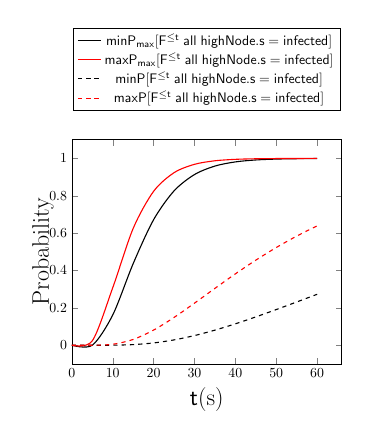
\begin{tikzpicture}[scale=0.5]

\begin{axis}[legend style={at={(0.5,1.5)},
        anchor=north},
        xlabel={\LARGE {\sf t}(s)},
        ylabel={\LARGE Probability},
        ylabel style={yshift=-0.35cm},
        xmin=0]
    \addplot[smooth,color=black,mark=none,thick] coordinates {
    (0,0)
    (5,0)
    (10,0.16168191528320316)
    (15,0.43664354895798035)
    (20,0.6720029347952551)
    (25,0.82610800015151)
    (30,0.9136074702688929)
    (35,0.9590691360474696)
    (40,0.9812970327955056)
    (45,0.9916939964155853)
    (50,0.9963953546920137)
    (55,0.99846517259443)
    (60,0.9993568735327532)
    };
\addlegendentry{{\normalsize ${\sf minP_{max} [F^{\leq t} \; all \; highNode.s=infected]}$}}

\addplot[smooth,color=red,mark=none,thick] coordinates {
(0,0)
(5,0.0234375)
(10,0.3074493408203125)
(15,0.6250644400715828)
(20,0.8237817112240009)
(25,0.9235288491465141)
(30,0.9683879644098142)
(35,0.9873372074679062)
(40,0.9950359542133387)
(45,0.9980839887961112)
(50,0.9992690485518201)
(55,0.9997236775734806)
(60,0.9998963078297327)
};
\addlegendentry{{\normalsize ${\sf maxP_{max} [F^{\leq t} \; all \; highNode.s=infected]}$}}


   \addplot[smooth,color=black,mark=none,thick, dashed] coordinates {
    (0,0)
    (5,0)
    (10,0.0002799)
    (15,0.0032855362005644244)
    (20,0.012245051235991131)
    (25,0.02848561456678314)
    (30,0.05170065872895695)
    (35,0.08081420233387326)
    (40,0.11453015780018033)
    (45,0.1515943815756742)
    (50,0.1908979081084969)
    (55,0.23150461747340917)
    (60,0.27264629297688076)
    
    };
\addlegendentry{{\normalsize ${\sf minP [F^{\leq t} \; all \; highNode.s=infected]}$}}

\addplot[smooth,color=red,mark=none,thick, dashed] coordinates {
(0,0)
(5,0.00001)
(10,0.004970004963101317)
(15,0.030891830831674055)
(20,0.08111415272896076)
(25,0.14860668504946992)
(30,0.22516767524651715)
(35,0.30439050974051723)
(40,0.3819645763513513)
(45,0.4552645658781883)
(50,0.5228635513529234)
(55,0.584136141072542)
(60,0.6389708133149984)
};
\addlegendentry{{\normalsize ${\sf maxP [F^{\leq t} \; all \; highNode.s=infected]}$}}

    \end{axis}

\end{tikzpicture}
\end{minipage}

&

\begin{minipage}{0.5\linewidth}
 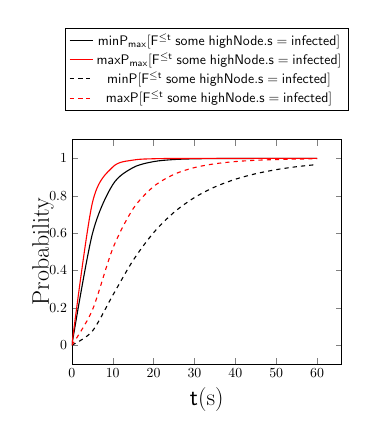
\begin{tikzpicture}[scale=0.5]

\begin{axis}[legend style={at={(0.5,1.5)},
        anchor=north},
        xlabel={\LARGE {\sf t}(s)},
        ylabel={\LARGE Probability},
        ylabel style={yshift=-0.35cm},
        xmin=0]
    \addplot[smooth,color=black,mark=none,thick] coordinates {
    (0,0)
    (5,0.59374609375)
    (10,0.859298205029335)
    (15,0.9511403067851839)
    (20,0.9829996663026497)
    (25,0.9940717986984359)
    (30,0.9979281926336163)
    (35,0.9992744402616341)
    (40,0.9997454403022622)
    (45,0.9999105517273437)
    (50,0.99999)
    (55,0.99999)
    (60,0.99999)
    };
\addlegendentry{{\normalsize ${\sf minP_{max} [F^{\leq t} \; some \; highNode.s=infected]}$}}

\addplot[smooth,color=red,mark=none,thick] coordinates {
    (0,0)
    (5,0.759765625)
    (10,0.9537906646728516)
    (15,0.9911339376121759)
    (20,0.9982989453365008)
    (25,0.9996736334872285)
    (30,0.9999373829057612)
    (35,0.9999879862046587)
    (40,0.9999976950179459)
    (45,0.9999995577632114)
    (50,0.999999)
    (55,0.999999)
    (60,0.999999)
};
\addlegendentry{{\normalsize ${\sf maxP_{max} [F^{\leq t} \; some \; highNode.s=infected]}$}}


   \addplot[smooth,color=black,mark=none,thick, dashed] coordinates {
    (0,0)
    (5,0.07482214356016052)
    (10,0.2666195786024801)
    (15,0.45468287053365297)
    (20,0.6026290596278729)
    (25,0.711698353836562)
    (30,0.7905821177345737)
    (35,0.847436872683398)
    (40,0.888500012673573)
    (45,0.9182713671810907)
    (50,0.9399436518334022)
    (55,0.9557785812955425)
    (60,0.9673849744323177)

    };
\addlegendentry{{\normalsize ${\sf minP [F^{\leq t} \; some \; highNode.s=infected]}$}}

\addplot[smooth,color=red,mark=none,thick, dashed] coordinates {
    (0,0)
    (5,0.1869973037081353)
    (10,0.516867492927023)
    (15,0.7308760605884067)
    (20,0.8495643000170283)
    (25,0.9147278419365144)
    (30,0.950991431198855)
    (35,0.9715044897471008)
    (40,0.9832788857161667)
    (45,0.9901188534628129)
    (50,0.9941299517108645)
    (55,0.9964991745411755)
    (60,0.9979061960860671)
};
\addlegendentry{{\normalsize ${\sf maxP [F^{\leq t} \; some \; highNode.s=infected]}$}}

    \end{axis}

\end{tikzpicture}
\end{minipage}


\end{tabular}

    \caption{Network virus infection results}
    \label{fig:virusresults}
\end{figure}

\subsubsection{Tele-Assistance System (TAS)}
\label{sec:tas}

The goal of the TAS exemplar system~\cite{DBLP:conf/icse/WeynsC15} is tracking a patient's vital parameters to adapt drug type or dose when needed, and taking actions in case of emergency.
TAS combines three service types in a workflow (Figure~\ref{fig:tas}).

\begin{figure}[!htbp]
    \centering
    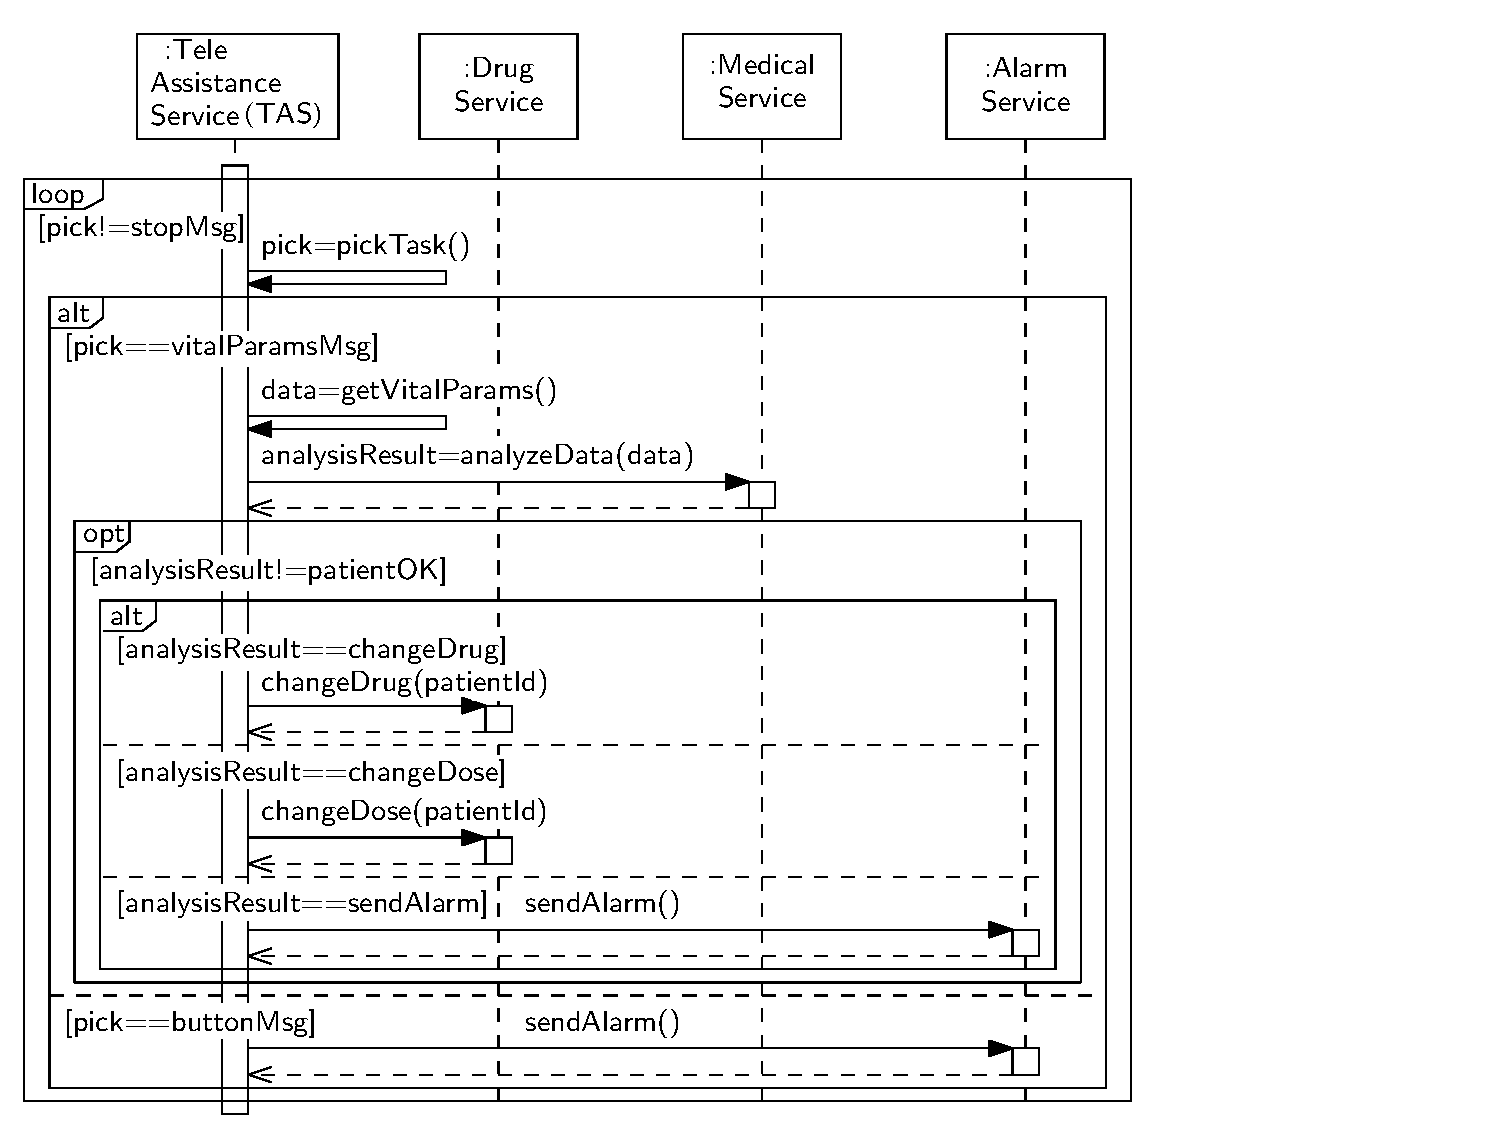
\includegraphics[width=0.8\linewidth]{figures/taswf}    
    \caption{Tele assistance service workflow} %(adapted from~\cite{DBLP:conf/icse/WeynsC15})}
    \label{fig:tas}      
    %\vspace{-0.2cm}
\end{figure}

When TAS receives a request that includes the vital parameters of a patient, its {\em Medical Service} analyzes the data and replies with instructions to: (i)~change the patient's drug type, (ii)~change the drug dose, or (iii)~trigger an alarm for first responders in case of emergency.
When changing the drug type or dose, TAS notifies a local pharmacy using a {\em Drug Service}, whereas first responders are notified via an {\em Alarm Service}.

\smallskip
The following excerpt shows the TAS workflow modeled as a signature in which static fields correspond to service bindings, and its behavior specification defines a set of local variables that keep track of the workflow status:
%\smallskip
%\noindent\rule[0.5ex]{\linewidth}{1pt}

{\scriptsize
\begin{Verbatim}[commandchars=\\\{\},codes={\catcode`$=3\catcode`^=7\catcode`_=8}]
\color{blue}one sig \color{black}TASWorkflow \{MSBindings: \color{blue}some \color{black}MedicalAnalysisService, 
\;\;\;\;\;\;\;\;\;\;\;\;\;\;\;\;\;\;\;\;\;\;\;\;\;\;\;\;\;\;\;\;\;\; ... ASBindings: \color{blue}some \color{black}AlarmService\}
\color{red}</ \color{blue}enum \color{black}tasks:\{notSelected, getVitalParams, buttonMsg\};
   \color{blue}enum \color{black}analysisResultTypes:\{none, patientOK, ...sendAlarm\};
   \color{blue}var \color{black}task:[tasks] \color{blue}init \color{black}notSelected; ...
   \color{blue}var \color{black}MSInvoked, workflowOK, workflowDone: \color{blue}bool init false\color{black};
   [pickTask] (task=notSelected) -> \color{prismgreen}//PickTask
      0.5: (task'=getVitalParams) + 0.5: (task'=buttonMsg);
   [] (task=buttonMsg) & (!MSInvoked) -> 
      (MSInvoked'=true) & (analysisResult'=sendAlarm); 
   [MSBindings:analyzeData] (task=getVitalParams) & 
   (!MSInvoked) -> (MSInvoked'=true); \color{prismgreen}
   [MSBindings:analysisResultPatientOK]  (MSInvoked) -> 
      (analysisResult'=patientOK) & (workflowOK'=\color{blue}true\color{black}) 
    & (workflowDone'=\color{blue}true\color{black}); ...
   [MSBindings:analysisResultSendAlarm]  (MSInvoked) -> 
      (analysisResult'=sendAlarm); ...
   [MSBindings:timeout] (timeouts=0) & (MSInvoked) -> 
      (workflowDone'=\color{blue}true\color{black}); ... \color{red}/>
\end{Verbatim}
}
%\smallskip

Calls to service operations are prefixed by the service binding relation (e.g., {\tt analyzeData} is prefixed by {\tt MSBinding}), so that the actual binding between the workflow and the services will be automatically created by the tool when configurations are generated.

The functionality of each service type in TAS is provided by third parties with different levels of performance, reliability, and cost (Table~\ref{tab:providers}). The metrics employed for the quality attributes are the percentage of service failures for reliability, and service response time for performance.
Service providers can be created as abstract signatures that encode these attributes as formulas, and include a constraint to include a binding on the service side to the workflow:

%\noindent\rule[0.5ex]{\linewidth}{1pt}
{\scriptsize
\begin{Verbatim}[commandchars=\\\{\},codes={\catcode`$=3\catcode`^=7\catcode`_=8}]
\color{blue}abstract sig \color{black}ServiceProvider \{WorkflowBinding: \color{blue}one \color{black}TASWorkflow\}
\color{blue}fact \color{black}\{\color{blue}all \color{black}sp:ServiceProvider, w:TASWorkflow | 
   sp \color{blue}in \color{black}w.ServiceBindings <=> w=sp.WorkflowBinding\}
\color{red}</ \color{blue}formula \color{black}failure\_rate, response\_time, cost; \color{red}/>
\end{Verbatim}
}

Service providers are subtyped by the types of service involved in the composition. Service invocation includes two probabilistic outcomes that model the possibility of service failure:

%\noindent\rule[0.5ex]{\linewidth}{1pt}
{\scriptsize
\begin{Verbatim}[commandchars=\\\{\},codes={\catcode`$=3\catcode`^=7\catcode`_=8}]
\color{blue}abstract sig \color{black}MedicalAnalysisService \color{blue}extends \color{black}ServiceProvider \{\}
\color{red}</ \color{blue}var \color{black}serviceOK: \color{blue}bool init false\color{black};
   \color{blue}var \color{black}ready :\color{blue} bool init true\color{black};
   [WorkflowBinding:analyzeData] (ready) -> 
        failure\_rate: (serviceOK'=\color{blue}false\color{black}) & (ready'=\color{blue}false\color{black}) 
    + 1-failure\_rate: (serviceOK'=\color{blue}true\color{black}) & (ready'=\color{blue}false\color{black});
   [WorkflowBinding:analysisResultPatientOK](!ready) 
   & (serviceOK) -> (serviceOK'=\color{blue}false\color{black}) & (ready'=\color{blue}true\color{black}); ...
   \color{blue}reward \color{black}costRew [WorkflowBinding:analyzeData] \color{blue}true\color{black} : cost;
   \color{blue}reward \color{black}timeRew [WorkflowBinding:analysisResultPatientOK]
   \color{blue}true\color{black} : response\_time; \color{red}/>
\end{Verbatim}
}

Every concrete service extends a service type encoded with a set of attribute values. 
The use of the quantifier {\tt lone} indicates that the use of every instance is optional, giving flexibility to use alternative services of the same type in the composition: 
%\noindent\rule[0.5ex]{\linewidth}{1pt}

{\scriptsize
\begin{Verbatim}[commandchars=\\\{\},codes={\catcode`$=3\catcode`^=7\catcode`_=8}]
\color{blue}lone sig \color{black}MS1 \color{blue}extends \color{black}MedicalAnalysisService\{\}
\color{red}</ \color{blue}formula \color{black}failure\_rate=0.06, response\_time=22, cost=9.8; \color{red}/>
\end{Verbatim}
}

\begin{table}[!hbt]
%\vspace{-0.3cm}
\centering
\caption{Properties of TAS service providers}
%\vspace{-0.1cm}
\setlength\tabcolsep{4pt}
{\scriptsize
\bgroup
\def\arraystretch{0.60}
\begin{tabular}{ccccc}
\toprule
Service & Name & Fail. rate (\%) & Resp.time (ms) & Cost (usd) \\
% &  & (\%) & (ms.) & (usd) \\
\midrule
MS1 & Medical Service 1 & 0.06 & 22 & 9.8 \\
MS2 & Medical Service 2 & 0.1 & 27 & 8.9 \\
MS3 & Medical Service 3 & 0.15 & 31 & 9.3 \\
MS4 & Medical Service 4 & 0.25 & 29 & 7.3 \\
MS5 & Medical Service 5 & 0.05 & 20 & 11.9 \\
\midrule
AS1 & Alarm Service 1 & 0.3 & 11 & 4.1 \\
AS2 & Alarm Service 2 & 0.4 & 9 & 2.5 \\
AS3 & Alarm Service 3 & 0.08 & 3 & 6.8 \\
\midrule
D1 & Drug Service & 0.12 & 1 & 0.1 \\
\bottomrule
\end{tabular}
\egroup
}
\vspace{0.3cm}

\label{tab:providers}
\end{table}

Finding an adequate design for the system entails understanding the tradeoff space by finding the set of system configurations that satisfy: (i)~structural constraints, e.g., the {\em Drug Service} must not be connected to an {\em Alarm Service}, (ii)~behavioral correctness properties (e.g., the system is eventually going to provide a response -- either by dispatching an ambulance or notifying a change to the pharmacy), and (iii)~quality requirements, which can be formulated as a combination of quantitative constraints and optimizations, e.g.:
(R1)~The average failure rate must not exceed {\tt fr} \%, 
(R2)~The average response time must not exceed {\tt rt} ms, and 
(R3)~Subject to R1 and R2, the cost should be minimized.

% \begin{table}[!h]
% %\vspace{-0.3cm}
% \centering
% \caption{Example of quality requirements for TAS}
% %\vspace{-0.1cm}
% \setlength\tabcolsep{10pt}
% {\footnotesize
% \bgroup
% \def\arraystretch{0.70}
% \begin{tabular}{ll}
% \toprule
% Name & Description\\
% \midrule
% R1 & The average failure rate should not exceed {\tt fr} \%.\\
% R2 & The average response time should not exceed {\tt rt} ms.\\
% R3 & Subject to R1 and R2, the cost should be minimized.\\
% \bottomrule
% \end{tabular}
% \egroup
% }
% %\vspace{-0.2cm}
% %\vspace{0.1cm}
% \label{tab:qreqs}
% \end{table}


%\smallskip
%An example of a set of quality requirements for TAS in this scenario might be the following:\\
%\indent R1. The average failure rate should not exceed 0.03\%.\\
%\indent R2. The average response time should not exceed 26 ms.\\
%\indent R3. Subject to R1 and R2, the cost should be minimized.\\
%\smallskip

%Generalizing from the concrete TAS scenario, the problem that we try to solve is: 
%{\em Find a system configuration that maintains a desired level of quality for multiple goals and optimize the solution according to another goal}.

%Exploring the design space to find the best possible configurations that conform to the architectural rules of TAS goes beyond the mere instantiation of components, and entails flexibility when envisaging design alternatives that may not always be obvious to a human designer (e.g., allowing invocation of multiple alarm services concurrently to reduce the response time and increase the reliability at the expense of additional cost).
We can automatically search the design space to find the best legal configurations with respect to these requirements by checking the composite M-PCTL property {\sf constrained\_cost}:

{\footnotesize
\smallskip
\centerline{${\sf reliable \equiv SallP_{\leq fr} [F \; some\; TASWorkflow.workFlowOK]}$}
\smallskip
\centerline{${\sf performant \equiv SallR^{timeRew}_{\leq rt} [F \; some\; TASWorkflow.workFlowDone]}$}
\smallskip
\centerline{${\sf mincost \equiv minR^{costRew} [F \; some\; TASWorkflow.workFlowDone]}$}
\smallskip
\centerline{${\sf constrained\_mincost \equiv \langle reliable \cap performant\rangle \; mincost}$}
\smallskip
}

The formulas labeled as {\sf reliable} and {\sf performant} obtain the set of configurations that satisfy the reliability and performance requirements {\sf R1} and {\sf R2}, respectively. 
Then, we can quantify the minimum cost entailed by these joint requirements by scoping the quantification of the third property {\sf mincost} to the subset of designs that satisfy the first two properties. 
For obtaining the configuration(s) that minimize cost for the specified performance and reliability levels, we substitute the quantifier in {\sf mincost} by {\sf SminR}.%., and compute:

%\centerline{${\sf confs\_mincost \equiv  reliable \cap performant\ \cap \; mincost}$.}

% TAS Analysis results
\begin{figure}
\centering
\begin{tabular}{ccc}

\begin{minipage}{0.5\linewidth}
 \begin{tikzpicture}[scale=0.5]
    \begin{axis}[x dir = reverse, y dir = reverse,colormap name=hot,
     xlabel={\large{Reliability (\%)}},
     ylabel={\large{Response time (ms.)}},
     zlabel={\large{Cost (usd)}},
     ylabel style={yshift=0.25cm, xshift=0.1cm, rotate=40},
     xlabel style={yshift=0.2cm, rotate=0},
     zlabel style={yshift=-0.2cm, rotate=0}     
     ]

    \addplot3 [surf, mesh/cols=20, z buffer=sort, restrict z to domain=0:inf, shader=faceted interp] shell {
    echo "
        data=dlmread('figures/data-tas/data.txt');
        res=\pgfkeysvalueof{/pgfplots/mesh/cols};
        [xx,yy] = meshgrid(linspace(min(data(:,1)), max(data(:,1)),res), linspace(min(data(:,2)), max(data(:,2)),res));
        zz=griddata(data(:,1),data(:,2),data(:,3),xx,yy);
        zz(isnan(zz))=-999;
        disp([xx(:) yy(:) zz(:)])
    " | octave --silent};   
    
    \end{axis}
    \end{tikzpicture}
\end{minipage}

& \hspace{-0.5cm} &

\begin{minipage}{0.5\linewidth}
    \begin{tikzpicture}[scale=0.5]
        \begin{axis}[cycle list name=BrBG, x dir = reverse, y dir = reverse,
        ylabel style={yshift=-0.6cm},
        xlabel={\large{Reliability (\%)}},
        ylabel={\large{Response time (ms.)}}]
        \addplot [no markers, fill=BrBG-A] table{figures/data-tas/map/sol_83.dat};
        \addplot [no markers, fill=BrBG-B] table{figures/data-tas/map/sol_87.dat};
        \addplot [no markers, fill=BrBG-C] table{figures/data-tas/map/sol_64.dat};
        \addplot [no markers, fill=BrBG-D] table{figures/data-tas/map/sol_61.dat};
        \addplot [no markers, fill=BrBG-E] table{figures/data-tas/map/sol_62.dat};
        \addplot [no markers, fill=BrBG-F] table{figures/data-tas/map/sol_9.dat};
        \addplot [no markers, fill=BrBG-G] table{figures/data-tas/map/sol_0.dat};
        \addplot [no markers, fill=BrBG-H] table{figures/data-tas/map/sol_1.dat};
        \addplot [no markers, fill=BrBG-I] table{figures/data-tas/map/sol_32.dat};
        \addplot [no markers, fill=BrBG-J] table{figures/data-tas/map/sol_30.dat};
        \addplot [no markers, fill=BrBG-K] table{figures/data-tas/map/sol_31.dat};
        \addplot [no markers, fill=BrBG-L] table{figures/data-tas/map/sol_15.dat};
        \addplot [no markers, fill=BrBG-M] table{figures/data-tas/map/sol_10.dat};
        \addplot [no markers, fill=BrBG-N] table{figures/data-tas/map/sol_58.dat};
        \addplot [no markers, fill=BrBG-O] table{figures/data-tas/map/sol_78.dat};
        \addplot [no markers, fill=BrBG-A] table{figures/data-tas/map/sol_77.dat};
        \addplot [no markers, fill=BrBG-B] table{figures/data-tas/map/sol_74.dat};
        \addplot [no markers, fill=BrBG-C] table{figures/data-tas/map/sol_55.dat};
        \addplot [no markers, fill=BrBG-D] table{figures/data-tas/map/sol_70.dat};
        \addplot [no markers, fill=red] table{figures/data-tas/map/sol_47.dat};
        \addplot [no markers, fill=BrBG-F] table{figures/data-tas/map/sol_25.dat};
        \addplot [no markers, fill=BrBG-G] table{figures/data-tas/map/sol_42.dat};
        \addplot [no markers, fill=BrBG-H] table{figures/data-tas/map/sol_41.dat};
        \addplot [no markers, fill=BrBG-I] table{figures/data-tas/map/sol_28.dat};
        \end{axis}
    \end{tikzpicture}
\end{minipage}

\end{tabular}

    \caption{TAS analysis results}
    \label{fig:tasresults}
\end{figure}

Figure~\ref{fig:tasresults} shows analysis results. 
The plot on the left shows the minimized cost of configurations for different levels of constraints on response time and reliability. It was computed by checking property ${\sf constrained\_mincost}$ in the region of the state space in which ${\tt fr} \in [0.98,1]$ and ${\tt rt} \in [15,35]$. 
As expected, higher response times and lower reliability correspond to lower costs, whereas peaks in cost are reached with lowest failure rates and response times.

The plot on the right is a map that shows which configurations best satisfy design criteria. 
Out of the set of 90 configurations that can be generated for TAS, only 24 satisfy the criteria in some subregion of the state space. 
If we consider that designers are interested e.g., in systems with response times  $\leq$26ms, and with a reliability of $\geq$99\%, we can determine which are the configurations that best satisfy constraints by checking ${\sf confs\_mincost}$ with ${\tt rt}=26$ and ${\tt fr}=0.01$ (highlighted in red in the figure).

Designers can take these results and make informed design decisions based, for instance, on the available budget for the project and legal constraints on the level of reliability and timeliness demanded of systems for first-aid response.

\subsubsection{Distributed Self-Protecting System}
\label{sec:cas}

Some large-scale systems are composed of federated entities that use self-adaptation to improve their behavior with respect to defined quality standards.
For example, Netflix's software infrastructure includes deployments in multiple regions controlled by a local manager (Scryer) to provision the resources required for maintaining resilience against changing customer traffic~\cite{meshenberg, jacobson}.

We apply our approach on a model of a Collective Adaptive System (CAS) with similar cooperative systems that defend against an external attack (e.g., DoS). 
We analyze the resilience that results from the selection of different communication topologies to disseminate security information for preemptive adaptation, quantified as the probability that all members of the CAS survive the attack. 

In the scenario~\cite{caspubh}, an external attacker uses a defined amount of available resources to attempt to breach members of the CAS (e.g., by placing a high number of requests). 
Each CAS member has the ability to detect the attack, defend itself against it by employing a fixed set of defense resources, and has the ability to notify other members of the CAS of the attack. Once a CAS member is notified, it will adapt and become invulnerable to the attempted breach.  
 
 {\scriptsize
 \begin{Verbatim}[commandchars=\\\{\},codes={\catcode`$=3\catcode`^=7\catcode`_=8}]
 \color{blue}some sig \color{black}sam \{conn: \color{blue}some \color{black}sam, attackVector: \color{blue}one \color{black}attacker\}
\color{red}</ \color{blue}enum \color{black}modes:\{normal, attackDetected, compromised, adapted\};
   \color{blue}var \color{black}status:[modes] \color{blue}init \color{black}normal; ... \color{blue}formula \color{black}detect;
   \color{prismgreen}//attacked
   [attackVector:attack] (resources>0) & (status=normal) -> 
          detect: (status'=attackDetected) 
                & (resources'=deplete); 
      + 1-detect: (status'=normal) & (resources'=deplete);
   \color{prismgreen}//notify attack
   [conn:alert] (status=attackDetected) -> \color{blue}true\color{black}; 
   \color{prismgreen}//adapt if attack detected (or notified)
   [] (resources>0) & (status=attackDetected) -> 
      (status'=adapted);
   \color{prismgreen}//receive alert
   [conn:alert] (resources>0) & (status=normal) ->
         CHANNEL\_RELIABILITY: (status'=attackDetected)
     + 1-CHANNEL\_RELIABILITY: (status'=normal); 
   [] (resources=0) -> (status'=compromised); \color{red}/>
\end{Verbatim}
}

The excerpt above shows the basic encoding of a local self-adaptive manager (signature {\tt sam}). 
Environmental and system conditions, such as the reliability of communication channels and the sensitivity of detection mechanisms, can play an important role in the emergent behavior of the CAS and are explicitly captured by parameters that affect the outcome of certain actions (e.g., constant {\tt CHANNEL\_RELIABILITY} limits the ability of a local manager to be notified of an attack by other managers, whereas formula {\tt detect} encodes the probability that a {\tt sam} will detect the attack).

We can create models with different communication topologies by encoding a basic set of constraints that impose a connected network without self-loops and with symmetric relations:

{\scriptsize
 \begin{Verbatim}[commandchars=\\\{\},codes={\catcode`$=3\catcode`^=7\catcode`_=8}]
 (\color{blue}all \color{black}s:sam | sam \color{blue}in \color{black}s.*conn)
 \color{blue}and\color{black} (\color{blue}no iden\color{black} & conn) \color{blue}and \color{black}(conn = ~conn)
\end{Verbatim}
}

And then add extra constraints like the ones shown on the right of Figure~\ref{fig:topologyresults} for each one of the topologies to encode.

We can reason about the resilience of the CAS by encoding a property that determines the topologies with the highest chance of attack survival: ${\sf resilience \equiv maxP [F \; all\; sam.status=adapted]}$.

%{\footnotesize
%\centerline{${\sf resilience \equiv maxP [F \; all\; sam\!:\!status=adapted]}$}
%}

% CAS Analysis results
\begin{figure}[!htb]
\setlength{\tabcolsep}{0pt}
\begin{tabular}{cc}

\begin{minipage}{0.5\linewidth}
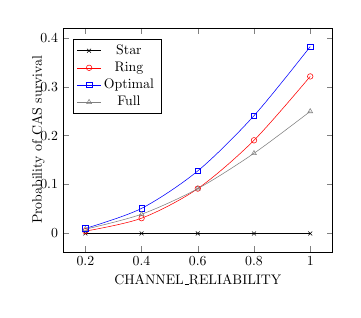
\begin{tikzpicture}[scale=0.5]

\begin{axis}[legend style={at={(0.2,0.95)},
		anchor=north},
		xlabel={\normalsize CHANNEL\_RELIABILITY},
		ylabel={\normalsize Probability of CAS survival},
		ylabel style={yshift=-0.35cm}]
	\addplot[smooth,color=black,mark=x] coordinates {
		(0.2,0)
		(0.4,0)
		(0.6,0)
		(0.8,0)
		(1,0)
	};
	\addlegendentry{{\normalsize Star}}
	\addplot[smooth,color=red,mark=o] coordinates {
		(0.2,0.00469)
		(0.4,0.031140)
		(0.6,0.091663)
		(0.8,0.190465)
		(1,0.32111)
	};
	\addlegendentry{{\normalsize Ring}}

	% \addplot[smooth,color=red,dashed] coordinates {
	% 	(0.2,0.00469)
	% 	(0.4,0.031140)
	% 	(0.6,0.091663)
	% 	(0.8,0.190465)
	% 	(1,0.32111)
	% };
	% \addlegendentry{{\normalsize Ring (WC)}}


	\addplot[smooth,color=blue,mark=square] coordinates {
		(0.2,0.010161)
		(0.4,0.05120538)
		(0.6,0.1278873)
		(0.8,0.240814)
		(1,0.38204905)
	};
	\addlegendentry{{\normalsize Optimal}}

	\addplot[smooth,color=gray,mark=triangle] coordinates {
		(0.2,0.00863437)
		(0.4,0.039317)
		(0.6,0.0916436)
		(0.8,0.16394455)
		(1,0.2496142)
	};
	\addlegendentry{{\normalsize Full}}


	\end{axis}

\end{tikzpicture}
\end{minipage}

& 

\begin{minipage}{0.5\linewidth}
{\footnotesize
\setlength{\tabcolsep}{0pt}
\bgroup
\def\arraystretch{0.70}
\begin{tabularx}{\linewidth}{>{\centering\arraybackslash}p{2cm}>{\centering\arraybackslash}p{2cm}}
\toprule
{\bf Full} & {\bf Star}\\
\midrule
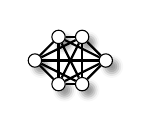
\begin{tikzpicture}[mynode/.style =  {draw,inner sep=0.6mm, circle,fill=white, blur shadow={shadow blur steps=3}} ,scale=0.15]

\node[mynode] (sam5) at (2,0) {};
\node[mynode] (sam1) at (0,2) {};
\node[mynode] (sam3) at (2,4) {};
\node[mynode] (sam2) at (4,4) {};
\node[mynode] (sam4) at (6,2) {};
\node[mynode] (sam0) at (4,0) {};

\begin{scope}[> = stealth,  -,black,thick, every node/.style = {black,right,align=center}]
%\draw (sam5) edge [left]   node     {}     (sam4);
%\draw (sam5) edge [left]   node     {}     (sam3);
%\draw (sam3) edge [left]   node     {}     (sam4);
%\draw (sam3) edge [left]   node     {}     (sam2);
%\draw (sam3) edge [left]   node     {}     (sam1);
%\draw (sam3) edge [left]   node     {}     (sam0);
\draw (sam3) edge [left]   node     {}     (sam5);
%\draw (sam0) edge [left]   node     {}     (sam4);
\draw (sam0) edge [left]   node     {}     (sam5);
%\draw (sam5) edge [left]   node     {}     (sam2);
\draw (sam0) edge [left]   node     {}     (sam1);
%\draw (sam5) edge [left]   node     {}     (sam1);
\draw (sam0) edge [left]   node     {}     (sam2);
%\draw (sam5) edge [left]   node     {}     (sam0);
\draw (sam0) edge [left]   node     {}     (sam3);
\draw (sam4) edge [left]   node     {}     (sam1);
\draw (sam4) edge [left]   node     {}     (sam0);
\draw (sam4) edge [left]   node     {}     (sam3);
\draw (sam4) edge [left]   node     {}     (sam2);
\draw (sam2) edge [left]   node     {}     (sam1);
\draw (sam2) edge [left]   node     {}     (sam0);
\draw (sam2) edge [left]   node     {}     (sam3);
\draw (sam2) edge [left]   node     {}     (sam5);
%\draw (sam2) edge [left]   node     {}     (sam4);
%\draw (sam1) edge [left]   node     {}     (sam2);
%\draw (sam1) edge [left]   node     {}     (sam0);
\draw (sam1) edge [left]   node     {}     (sam5);
\draw (sam1) edge [left]   node     {}     (sam3);
%\draw (sam1) edge [left]   node     {}     (sam4);
\draw (sam4) edge [left]   node     {}     (sam5);
\end{scope}
\end{tikzpicture}
 & 
\begin{tikzpicture}[mynode/.style =  {draw,inner sep=0.6mm, circle,fill=white, blur shadow={shadow blur steps=3}} ,scale=0.13]

\node[mynode] (sam5) at (1,0) {};
\node[mynode] (sam1) at (0,3) {};
\node[mynode] (sam3) at (3,2) {};
\node[mynode] (sam2) at (3,4.5) {};
\node[mynode] (sam4) at (6,3) {};
\node[mynode] (sam0) at (5,0) {};

\begin{scope}[> = stealth,  -,black,thick, every node/.style = {black,right,align=center}]
\draw (sam3) edge [left]   node     {}     (sam0);
\draw (sam3) edge [left]   node     {}     (sam1);
\draw (sam3) edge [left]   node     {}     (sam2);
\draw (sam3) edge [left]   node     {}     (sam4);
\draw (sam3) edge [left]   node     {}     (sam5);
\end{scope}
\end{tikzpicture} \\
\textcolor{blue}{all}  s:sam | \textcolor{blue}{all} s':sam-s | s \textcolor{blue}{in} s'.conn
& \textcolor{blue}{one} s:sam | s \textcolor{blue}{in} sam.conn \textcolor{blue}{and} \#(sam-s).conn=1 \\
\midrule
{\bf Ring} & {\bf Optimal}\\
\midrule
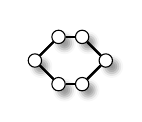
\begin{tikzpicture}[mynode/.style =  {draw,inner sep=0.6mm, circle,fill=white, blur shadow={shadow blur steps=3}} ,scale=0.15]

\node[mynode] (sam5) at (2,0) {};
\node[mynode] (sam1) at (0,2) {};
\node[mynode] (sam3) at (2,4) {};
\node[mynode] (sam2) at (4,4) {};
\node[mynode] (sam4) at (6,2) {};
\node[mynode] (sam0) at (4,0) {};

\begin{scope}[> = stealth,  -,black,thick, every node/.style = {black,right,align=center}]
\draw (sam3) edge [left]   node     {}     (sam2);
\draw (sam3) edge [left]   node     {}     (sam1);
\draw (sam0) edge [left]   node     {}     (sam4);
\draw (sam0) edge [left]   node     {}     (sam5);
\draw (sam5) edge [left]   node     {}     (sam1);
\draw (sam5) edge [left]   node     {}     (sam0);
\draw (sam4) edge [left]   node     {}     (sam0);
\draw (sam4) edge [left]   node     {}     (sam2);
\draw (sam2) edge [left]   node     {}     (sam3);
\draw (sam2) edge [left]   node     {}     (sam4);
\draw (sam1) edge [left]   node     {}     (sam5);
\draw (sam1) edge [left]   node     {}     (sam3);
\end{scope}
\end{tikzpicture} & 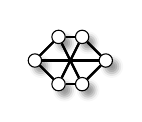
\begin{tikzpicture}[mynode/.style =  {draw,inner sep=0.6mm, circle,fill=white, blur shadow={shadow blur steps=3}} ,scale=0.15]

\node[mynode] (sam5) at (2,0) {};
\node[mynode] (sam1) at (0,2) {};
\node[mynode] (sam3) at (2,4) {};
\node[mynode] (sam2) at (4,4) {};
\node[mynode] (sam4) at (6,2) {};
\node[mynode] (sam0) at (4,0) {};

\begin{scope}[> = stealth,  -,black,thick, every node/.style = {black,right,align=center}]
\draw (sam3) edge [left]   node     {}     (sam2);
\draw (sam3) edge [left]   node     {}     (sam1);
\draw (sam3) edge [left]   node     {}     (sam0);
\draw (sam0) edge [left]   node     {}     (sam4);
\draw (sam0) edge [left]   node     {}     (sam5);
\draw (sam5) edge [left]   node     {}     (sam2);
\draw (sam5) edge [left]   node     {}     (sam1);
\draw (sam5) edge [left]   node     {}     (sam0);
\draw (sam0) edge [left]   node     {}     (sam3);
\draw (sam4) edge [left]   node     {}     (sam1);
\draw (sam4) edge [left]   node     {}     (sam0);
\draw (sam4) edge [left]   node     {}     (sam2);
\draw (sam2) edge [left]   node     {}     (sam3);
\draw (sam2) edge [left]   node     {}     (sam5);
\draw (sam2) edge [left]   node     {}     (sam4);
\draw (sam1) edge [left]   node     {}     (sam5);
\draw (sam1) edge [left]   node     {}     (sam3);
\draw (sam1) edge [left]   node     {}     (sam4);
\end{scope}
\end{tikzpicture}
 \\
\textcolor{blue}{all} s:sam | \#s.conn=2  & - \\
\bottomrule
\end{tabularx}
\egroup
}
\end{minipage}

\end{tabular}




\caption{CAS topologies and resilience results}
%\vspace{-0.5cm}
\label{fig:topologyresults}
\end{figure}

The left-hand side of Figure~\ref{fig:topologyresults} shows the resilience of the different topologies for values of channel reliability in the set \{0.2, 0.4, 0.6, 0.8, 1\}. 
As expected, all topologies present increased chances of survival with higher channel reliability, saving the star topology, for which resilience is always zero for the amount of {\tt sam} and attacker resources employed for the experiments (the central node is a weak link that hampers inter-node communication if compromised).
To obtain the optimal resilience (and its corresponding topology) for our scenario, we check the M-PCTL {\sf resilience} property, and an analogous property that employs the {\sf SmaxP} quantifier on a model that does not include any extra constraints. 


\subsection{Discussion}
Basing on our results, in this section we discuss the research questions posed in the introduction and threats to validity.
\subsubsection{(RQ1) Feasibility} We have shown that {\em raising the level of abstraction at which probabilistic models are described and queried can effectively enable joint reasoning about structural and quantitative guarantees of design spaces}. In terms of modeling, this is achieved by incorporating language constructs that allow structural relations to be referenced from elements of (probabilistic) behavioral specifications. In terms of analysis, incorporating novel quantifiers to check properties on collections of models in probabilistic temporal logics enables streamlined specification of sophisticated properties to study guarantees across the solution space.

%  We have shown that incorporating {\it modeling constructs that allow structural relations to be referenced from elements of (probabilistic) behavioral specifications and a language to check probabilistic temporal logic properties on collections of probabilistic models enables automated joint reasoning about the structure and stochastic behavior of sets of alternative system designs}. 
% Our prototype is based on constraint solving to synthesize structures and probabilistic model checking to analyze behaviors, although the languages and algorithm presented can be supported by alternative engines (e.g., SMT solver + statistical model checking).
\subsubsection{(RQ2) Generality} Our results show that {\it our approach is applicable to systems in different domains, in which uncertainty is introduced by disparate sources}.
Our approach is {\it particularly suited to problems in which structure/topology is relevant and multiple instances of similar, but different, components that exhibit probabilistic behavior (i.e., with different parameters or slight variations in behavior) interact in complex ways}. 
Moreover, we have shown that the approach can be applied to different analyses (average and best/worst case probabilities and rewards) and probabilistic formalisms (MDP and DTMC). This is effectively enabled by the fact HaiQ operates one level higher in the abstraction ladder, with respect to existing description languages in probabilistic model checking, and that the target language (PRISM) in which configuration behavioral models are generated (Step 2 in Figure~\ref{fig:overview}, implementing Algorithm~\ref{alg:cbg}) supports alternative underlying semantics for MDP and DTMC (c.f.~\cite{prismsemantics}). Similarly, M-PCTL extends PCTL, which can be naturally used to check properties both in DTMC and MDP. 

\subsubsection{(RQ3) Tradeoffs} \label{sec:tradeoffs} With respect to alternative approaches to analyze probabilistic behavior, {\sf HaiQ} comes with tradeoffs in terms of effort, reusability, computational cost, and analytical capabilities:

\smallskip 
\noindent {\em Effort.} In {\sf HaiQ}, structure and probabilistic behavior are expressed in a compact manner, and their combined analysis streamlined.
This contrasts with ad-hoc solutions that demand developing specific infrastructure and are error-prone. The analysis of a CAS scenario similar to the one in Section~\ref{sec:cas}~\cite{caspub} required combining the PRISM preprocessor~\cite{prismpp} with scripts that demanded topologies to be encoded as matrixes in separate text files, leading to multiple trial and error rounds (due to errors in matrix encodings, script tuning). 
For TAS, the problem has also been solved employing a custom template engine and a python script that generates probabilistic models based on analysis of Alloy specifications~\cite{taspub}. 
These solutions {\it required weeks of work, contrasting with a single-day specification effort (at most) required to solve the problem with {\sf HaiQ} in both cases}. 
Other approaches that do not include structural synthesis (e.g., direct specification in a model checker) require encoding explicitly all elements of every design alternative (e.g., topology), making it more error-prone and orders of magnitude more demanding than {\sf HaiQ} in terms of specification effort for non-trivial problems. 

\smallskip
\noindent{\em Reusability}. Compared to the ad-hoc solutions developed for the case studies presented, which required specific infrastructure, {\sf HaiQ} {\it provides an infrastructure that can be reused across a range of different domains}. 
Furthermore, {\it specifications in {\sf HaiQ} are also more reusable than those of existing probabilistic model checkers}, in which behavior types and communication topology are intertwined with the specific instances of processes. In contrast, behavioral type hierarchies can be reused as ``libraries'' across the same problem class in {\sf HaiQ}, since the specifics of instances are specified separately. 

\smallskip 
\noindent{\em Computational cost and analytical capabilities.} Prototype analysis performance behaves differently, depending on the problem type. 
In TAS, checking the compositional property {\sf constrained\_mincost} entailed exploring 90 configurations for an overall time of 6s ($\simeq$2\% was used for configuration synthesis).\footnote{Experiments were run on OSX10.1.5, Java 1.8.0\_111, 2.8GHz Core i7, 16GB RAM.}
Checking the {\sf resilience} property for a fixed topology in CAS took $\leq$40s in the worst case. However, checking for the optimal configuration took exploring 254 configurations ($\simeq$1hr, $\simeq$0.01\% used for synthesis). 
These numbers are explained by the low complexity of synthesis (few structural constraints to consider) relative to the possibly large number of configurations whose behavior has to be checked individually.
In any case, {\sf HaiQ} itself introduces a negligible overhead in analysis, and {\it is as efficient as the underlying verification technology that it employs} (backend engines capable of checking PCTL on PRISM models like STORM~\cite{DBLP:journals/corr/DehnertJK017} work out of the box). 
Anyway, it is worth noting that {\it the most computationally-demanding use cases of the approach correspond to analytical capabilities that did not exist in other approaches}, like obtaining the configurations that best satisfy a set of quantitative guarantees. 

\subsubsection{Threats to Validity}
\label{sec:threats} The approach is inspired by a specific style of relational description (Alloy) and behavioral formalisms (DTMC and MDP).
However, the constructs employed to formalize structures are fairly standard and synthesis of configurations is adaptable to other languages/models (e.g., OCL).
Concerning behavior descriptions, the fact that the approach was successfully instantiated for different probabilistic formalisms and analyses hints at feasibility of adapting the approach to other formalisms such as continuous-time Markov chains (CTMC) for finer-grained time analysis.
%or probabilistic timed automata (PTA) for finer-grained time analysis.
Focusing on {\em internal validity}, the degree of formal assurance on configurations provided by the approach is computationally expensive, and entails risks on the cost both of configuration synthesis and behavior analysis (derived from exploring potentially large state spaces of individual configuration behavior). 
These risks can be mitigated by exploiting the hierarchical relations that are naturally present in software designs, in which components interact in a structured way~\cite{DBLP:conf/sigsoft/KangMJ16}. Hence, synthesis of different subsystems with local constraints can be done independently and then composed, reducing the cost of configuration synthesis. 
This mitigation also allows parallelism in the analysis to be exploited, in which the behavior of configurations of subsystems can be independently analyzed in parallel~\cite{Johnson:2013:IVF:2465449.2465456}.  
Another risk derived from structural synthesis is that Alloy can generate additional isomorphic configurations that can add unnecessary computation time in some situations, although this does not affect the soundness of the results.

%Moreover, there are further reductions in analysis cost that can be obtained by identifying isomorphic configurations. 


\section{Conclusions and Future Work}
\label{sec:conclusion}

This paper introduces what is, to the best of our knowledge, the first approach that combines the advantages of relational modeling, structural synthesis, and quantitative verification. 
Our experience applying it in different domains shows that: (RQ1)~raising the level of abstraction by {\em (i)}~incorporating modeling constructs that allow structural relations to be referenced from elements of (probabilistic) behavioral specifications and {\em (ii)}~incorporating novel quantifiers to check properties across collections of models in probabilistic temporal logics, enables automated joint reasoning about structural and (probabilistic) quantitative guarantees across spaces of alternative system designs, (RQ2)~our approach is general enough to be applied to different probabilistic formalisms (DTMC and MDP), types of analyses (average and best/worst probability- and reward-based analysis), and domains where uncertainty is introduced by disparate sources, and (RQ3)~the approach brings new analytical capabilities to the validation of designs of software systems that operate under uncertainty, compared to existing quantitative verification approaches (e.g., automated identification of structural variants that optimize probability/reward-based guarantees). With respect to (RQ3), our experience and further logical arguments also point at reduction of specification effort and improved reusability with respect to existing probabilistic model checking techniques (c.f. Section~\ref{sec:tradeoffs}), although we still have to conduct an extensive study before we can consolidate our claims about these added benefits of the approach. We will perform this study in our next steps.

Concerning other future work, we plan to support alternative formalisms that allow reasoning about continuous-time (e.g., CTMC, PTA). Moreover, the approach is currently limited to analyzing behaviors within specific configurations, but is not able to reason about behaviors that imply structural changes. 
Future work will extend our approach to reason about such behaviors, and explore hierarchical specification~\cite{DBLP:conf/sigsoft/KangMJ16} and compositional verification~\cite{Johnson:2013:IVF:2465449.2465456} techniques (c.f., Section~\ref{sec:threats}) to improve modularity and scalability. 


% if have a single appendix:
%\appendix[Proof of the Zonklar Equations]
% or
%\appendix  % for no appendix heading
% do not use \section anymore after \appendix, only \section*
% is possibly needed

% use appendices with more than one appendix
% then use \section to start each appendix
% you must declare a \section before using any
% \subsection or using \label (\appendices by itself
% starts a section numbered zero.)
%


% \appendices
% \section{Proof of the First Zonklar Equation}
% Appendix one text goes here.

% % you can choose not to have a title for an appendix
% % if you want by leaving the argument blank
% \section{}
% Appendix two text goes here.


% % use section* for acknowledgment
% \ifCLASSOPTIONcompsoc
%   % The Computer Society usually uses the plural form
%   \section*{Acknowledgments}
% \else
%   % regular IEEE prefers the singular form
%   \section*{Acknowledgment}
% \fi


% The authors would like to thank...


% Can use something like this to put references on a page
% by themselves when using endfloat and the captionsoff option.
\ifCLASSOPTIONcaptionsoff
  \newpage
\fi



% trigger a \newpage just before the given reference
% number - used to balance the columns on the last page
% adjust value as needed - may need to be readjusted if
% the document is modified later
%\IEEEtriggeratref{8}
% The "triggered" command can be changed if desired:
%\IEEEtriggercmd{\enlargethispage{-5in}}

% references section

% can use a bibliography generated by BibTeX as a .bbl file
% BibTeX documentation can be easily obtained at:
% http://mirror.ctan.org/biblio/bibtex/contrib/doc/
% The IEEEtran BibTeX style support page is at:
% http://www.michaelshell.org/tex/ieeetran/bibtex/
\bibliographystyle{IEEEtran}
% argument is your BibTeX string definitions and bibliography database(s)
\bibliography{biblio}
%
% <OR> manually copy in the resultant .bbl file
% set second argument of \begin to the number of references
% (used to reserve space for the reference number labels box)
%\begin{thebibliography}{1}
%
%\bibitem{IEEEhowto:kopka}
%H.~Kopka and P.~W. Daly, \emph{A Guide to \LaTeX}, 3rd~ed.\hskip 1em plus
%  0.5em minus 0.4em\relax Harlow, England: Addison-Wesley, 1999.
%
%\end{thebibliography}

% biography section
% 
% If you have an EPS/PDF photo (graphicx package needed) extra braces are
% needed around the contents of the optional argument to biography to prevent
% the LaTeX parser from getting confused when it sees the complicated
% \includegraphics command within an optional argument. (You could create
% your own custom macro containing the \includegraphics command to make things
% simpler here.)
%\begin{IEEEbiography}[{\includegraphics[width=1in,height=1.25in,clip,keepaspectratio]{mshell}}]{Michael Shell}
% or if you just want to reserve a space for a photo:

\begin{IEEEbiography}[{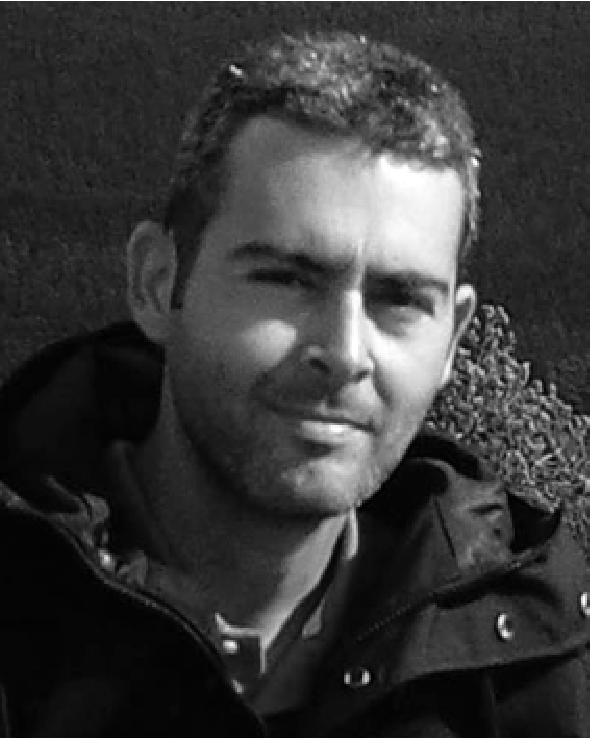
\includegraphics[width=1in,height=1.25in,clip,keepaspectratio]{jcamara.pdf}}]{Javier C\'{a}mara}
is a senior systems scientist at the Insitute for Software Research, Carnegie Mellon University. His research interests lie in the intersection of formal methods and software engineering, with a special interest in the areas of software engineering for self-adaptive systems, applied formal methods, and software architecture. 
\end{IEEEbiography}


% \begin{IEEEbiography}{Javier Camara}
% Biography text here.
% \end{IEEEbiography}

% % if you will not have a photo at all:
% \begin{IEEEbiographynophoto}{John Doe}
% Biography text here.
% \end{IEEEbiographynophoto}

% insert where needed to balance the two columns on the last page with
% biographies
%\newpage

%\begin{IEEEbiographynophoto}{Jane Doe}
%Biography text here.
%\end{IEEEbiographynophoto}

% You can push biographies down or up by placing
% a \vfill before or after them. The appropriate
% use of \vfill depends on what kind of text is
% on the last page and whether or not the columns
% are being equalized.

%\vfill

% Can be used to pull up biographies so that the bottom of the last one
% is flush with the other column.
%\enlargethispage{-5in}



% that's all folks
\end{document}


